\chapter[Results]{Results}

This chapter presents calculation results based on methodology described in Chapters 2 and 3. The effective multiplication factor, number density of major isotopes, and $^{232}$Th refill rate calculated using full-core model with 3-days step for a 20-year time frame. Moreover, radial and axial neutron flux, neutron flux energy spectrum, temperature reactivity coefficients, control rod worth, power density, and $^{233}$U breeding density distribution are presented for initial and equilibrium fuel salt composition. The neutron flux and energy spectrum are calculated for the full-core model, normalized by neutron lethargy and reported for each zone. The temperature coefficients of reactivity for both fuel salt and graphite are estimated at the initial state by comparing effective multiplication factors at a temperature values uniformly distributed from 900 K and 1000 K. The rod worth is calculated at several different insertion levels of graphite rods and safety rods. Finally, six factor analysis was performed to show those parameteres changing during reactor operation.

The neutron population per cycle, number of active/inactive cycles were chosen to obtain balance between reasonable tolerance for a transport problem ($\leq$ 40 pcm for effective multiplication factor) and computational time. The \gls{MSBR} depletion and safety parameters computations were performed on 64 Blue Waters' XK7 nodes (two AMD 6276 Interlagos CPU per node, 16 floating-point bulldozer core units per node or 32 ``integer" cores per node, nominal clock speed is 2.45 GHz). The total computational time for achieving equilibrium composition was about 9000 node hours (288'000 core hours.)

\section{Effective multiplication factor}
Figure~\ref{fig:keff} demonstrates the effective miltiplication factors obtained using SaltProc and SERPENT 2. The effective multiplication factors are calculated after removing fission products (table~\ref{tab:reprocessing_list}) and adding the fertile material at the end of ``cycle time" which was fixed at 3 days for this work. The \gls{MSBR} program defined a ``cycle time" as the amount of time required to remove 100\% of a target nuclide from a fuel salt. The effective multiplication factor significantly fluctuates because of descrete way to simulate online reprocessing. First, SERPENT 2 calculates effective multiplication factor for the beginning of cycle time (fresh fuel composition for the first step). Following this, it computes new fuel salt composition for the end of 3-day step and corresponding effective multiplication factor which is much smaller then previous one. Finally, SERPENT 2 calculates multiplication factor for the depleted composition after applying feeds and removals, and this value is significantly higher that one before reprocessing because major reactor poisons (e.g. Xe, Kr) were removed as well as fresh fissile material ($^{233}$U) from the protactinium decay tank was added. 

Additionaly, presence of rubidium, strontium, cesium, barium in the core has significant negative impact on reactor physics. In fact, removal of these elements every 3435 days causes multiplication factor jump by approximately 450 pcm, and limits using semi-batch approach for online reprocessing simulation. To avoid in future these fluctuations SERPENT 2 continuous online reprocessing procedure should be implemented. Overall, the effective multiplication factor gradually decreases from 1.075 to the equilibrium state with the factor about 1.02 after approximately 6 years of irradiation. 

The analysis of the fuel salt composition evolution provides more comprehensive information about the equilibrium state. Figure~\ref{fig:adens_eq} represents normalized by average atomic density of major nuclides which have strong influence on the reactor core physics, at the beginning of each depletion time step (before any feeds and removals). It could be noted that concentration of $^{233}$U, $^{232}$Th, $^{233}$Pa, $^{232}$Pa composition changes insignificantly after approximately 2500 days of operation. Particullarly, $^{233}$U number density fluctuation is less than 0.8\% in the time interval from 16 to 20 years of operation, hence, it might be assumed that quasi-equlibrium state was achieved after 16 years of the fuel salt irradiation.

\begin{figure}[htp!] % replace 't' with 'b' to 
  \centering
  \vspace{-0.3em}
  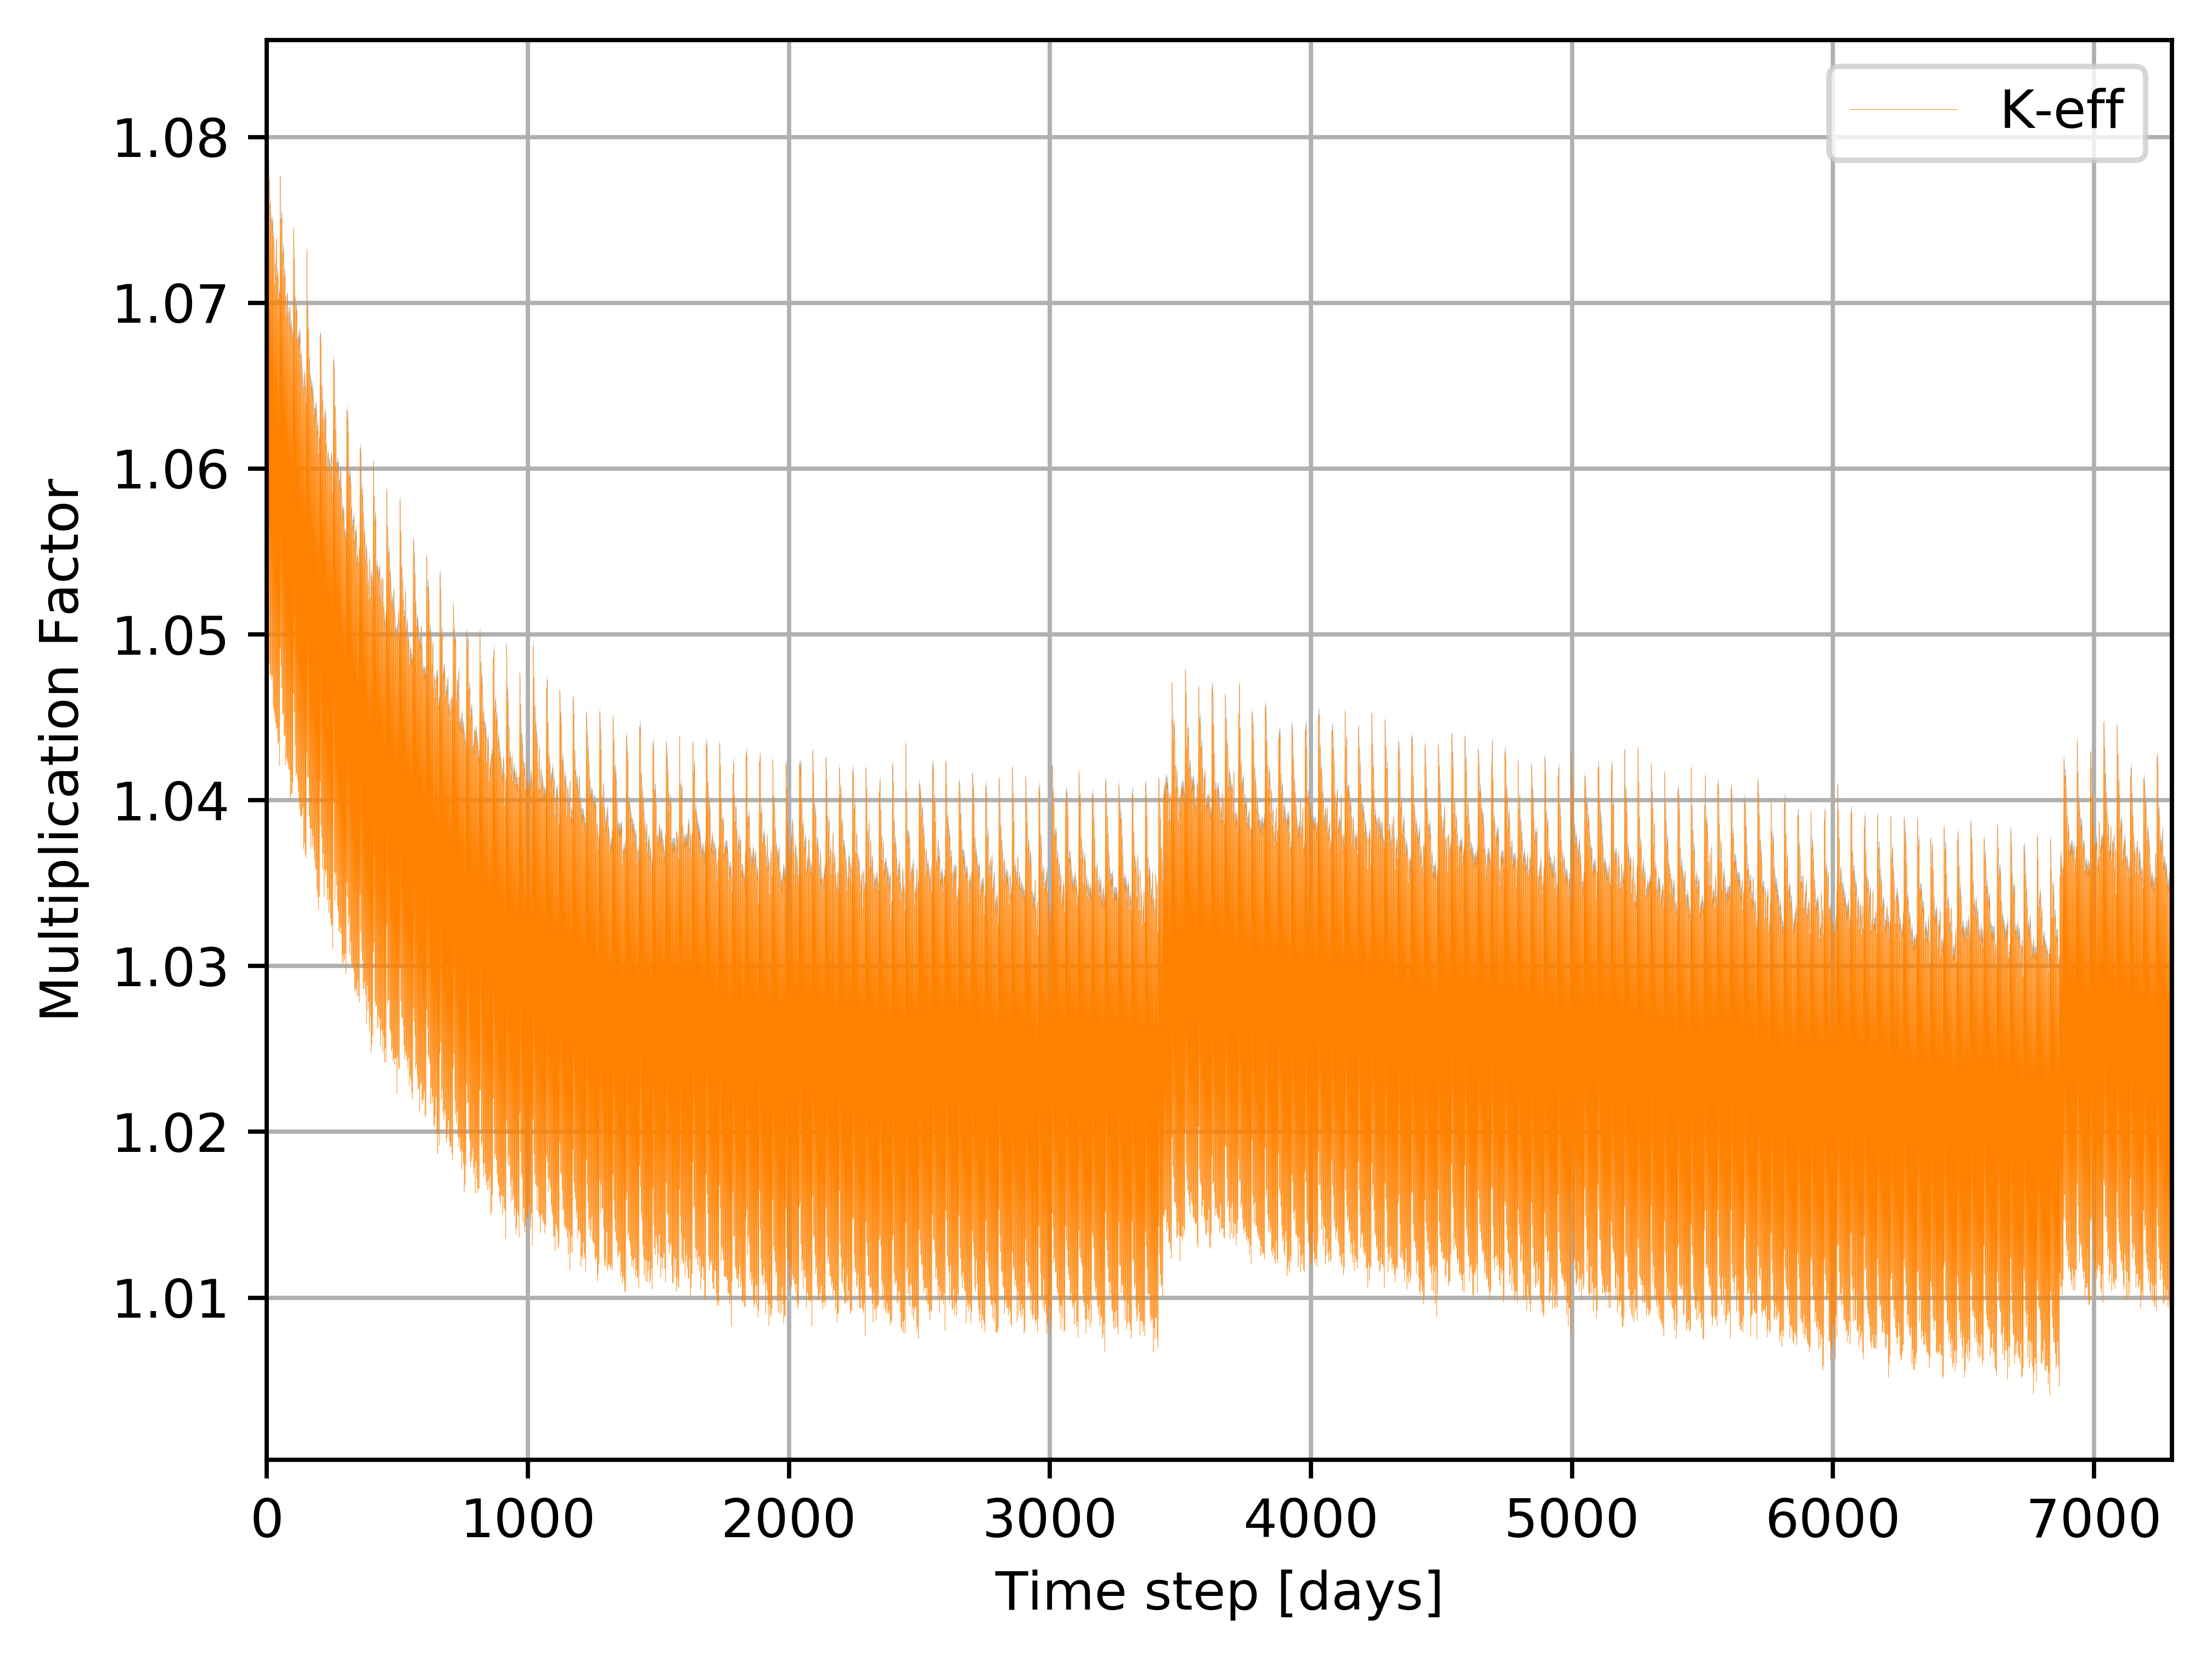
\includegraphics[width=1.05\textwidth]{keff.png}
  \caption{Effective multiplication factor dynamics for full-core \gls{MSBR} model for a 20-year reactor operation. The confidence interval $\pm\sigma$ is shaded.}
  \vspace{-0.6em}
  \label{fig:keff}
\end{figure}

In contrast, wide variety of nuclides, including fissile isotopes (e.g. $^{235}$U) and non-fissile strong absorbers (e.g. $^{234}$U), keep accumulating in the core. Figures~\ref{fig:fissile_short}, \ref{fig:fissile_long} demonstrates production of short-life and long-life fissile isotopes in the core. In the end of considered operational time significant amount of fissile $^{235}$U ($\approx 9\times10^{-6}$ atom/b-cm), $^{238}$Pu ($\approx 10^{-6}$ atom/b-cm), $^{237}$Np ($\approx10^{-6}$ atom/b-cm), $^{232}$U ($\approx$10$^{-7}$ atom/b-cm), $^{239}$Pu ($\approx10^{-7}$ atom/b-cm),$^{241}$Pu ($\approx 5\times10^{-8}$ atom/b-cm) while equilibrium number density of target fissile isotope $^{233}$U was about 7.97$\times10^{-5}$ atom/b-cm. Thus, production of new fissile materials in the core as well as $^{233}$U breeding make it possible to compensate negative effects of strong absorbers accumulation and keep the reactor critical.

\begin{figure}[htp!] % replace 't' with 'b' to 
  \centering
  \vspace{-0.3em}
  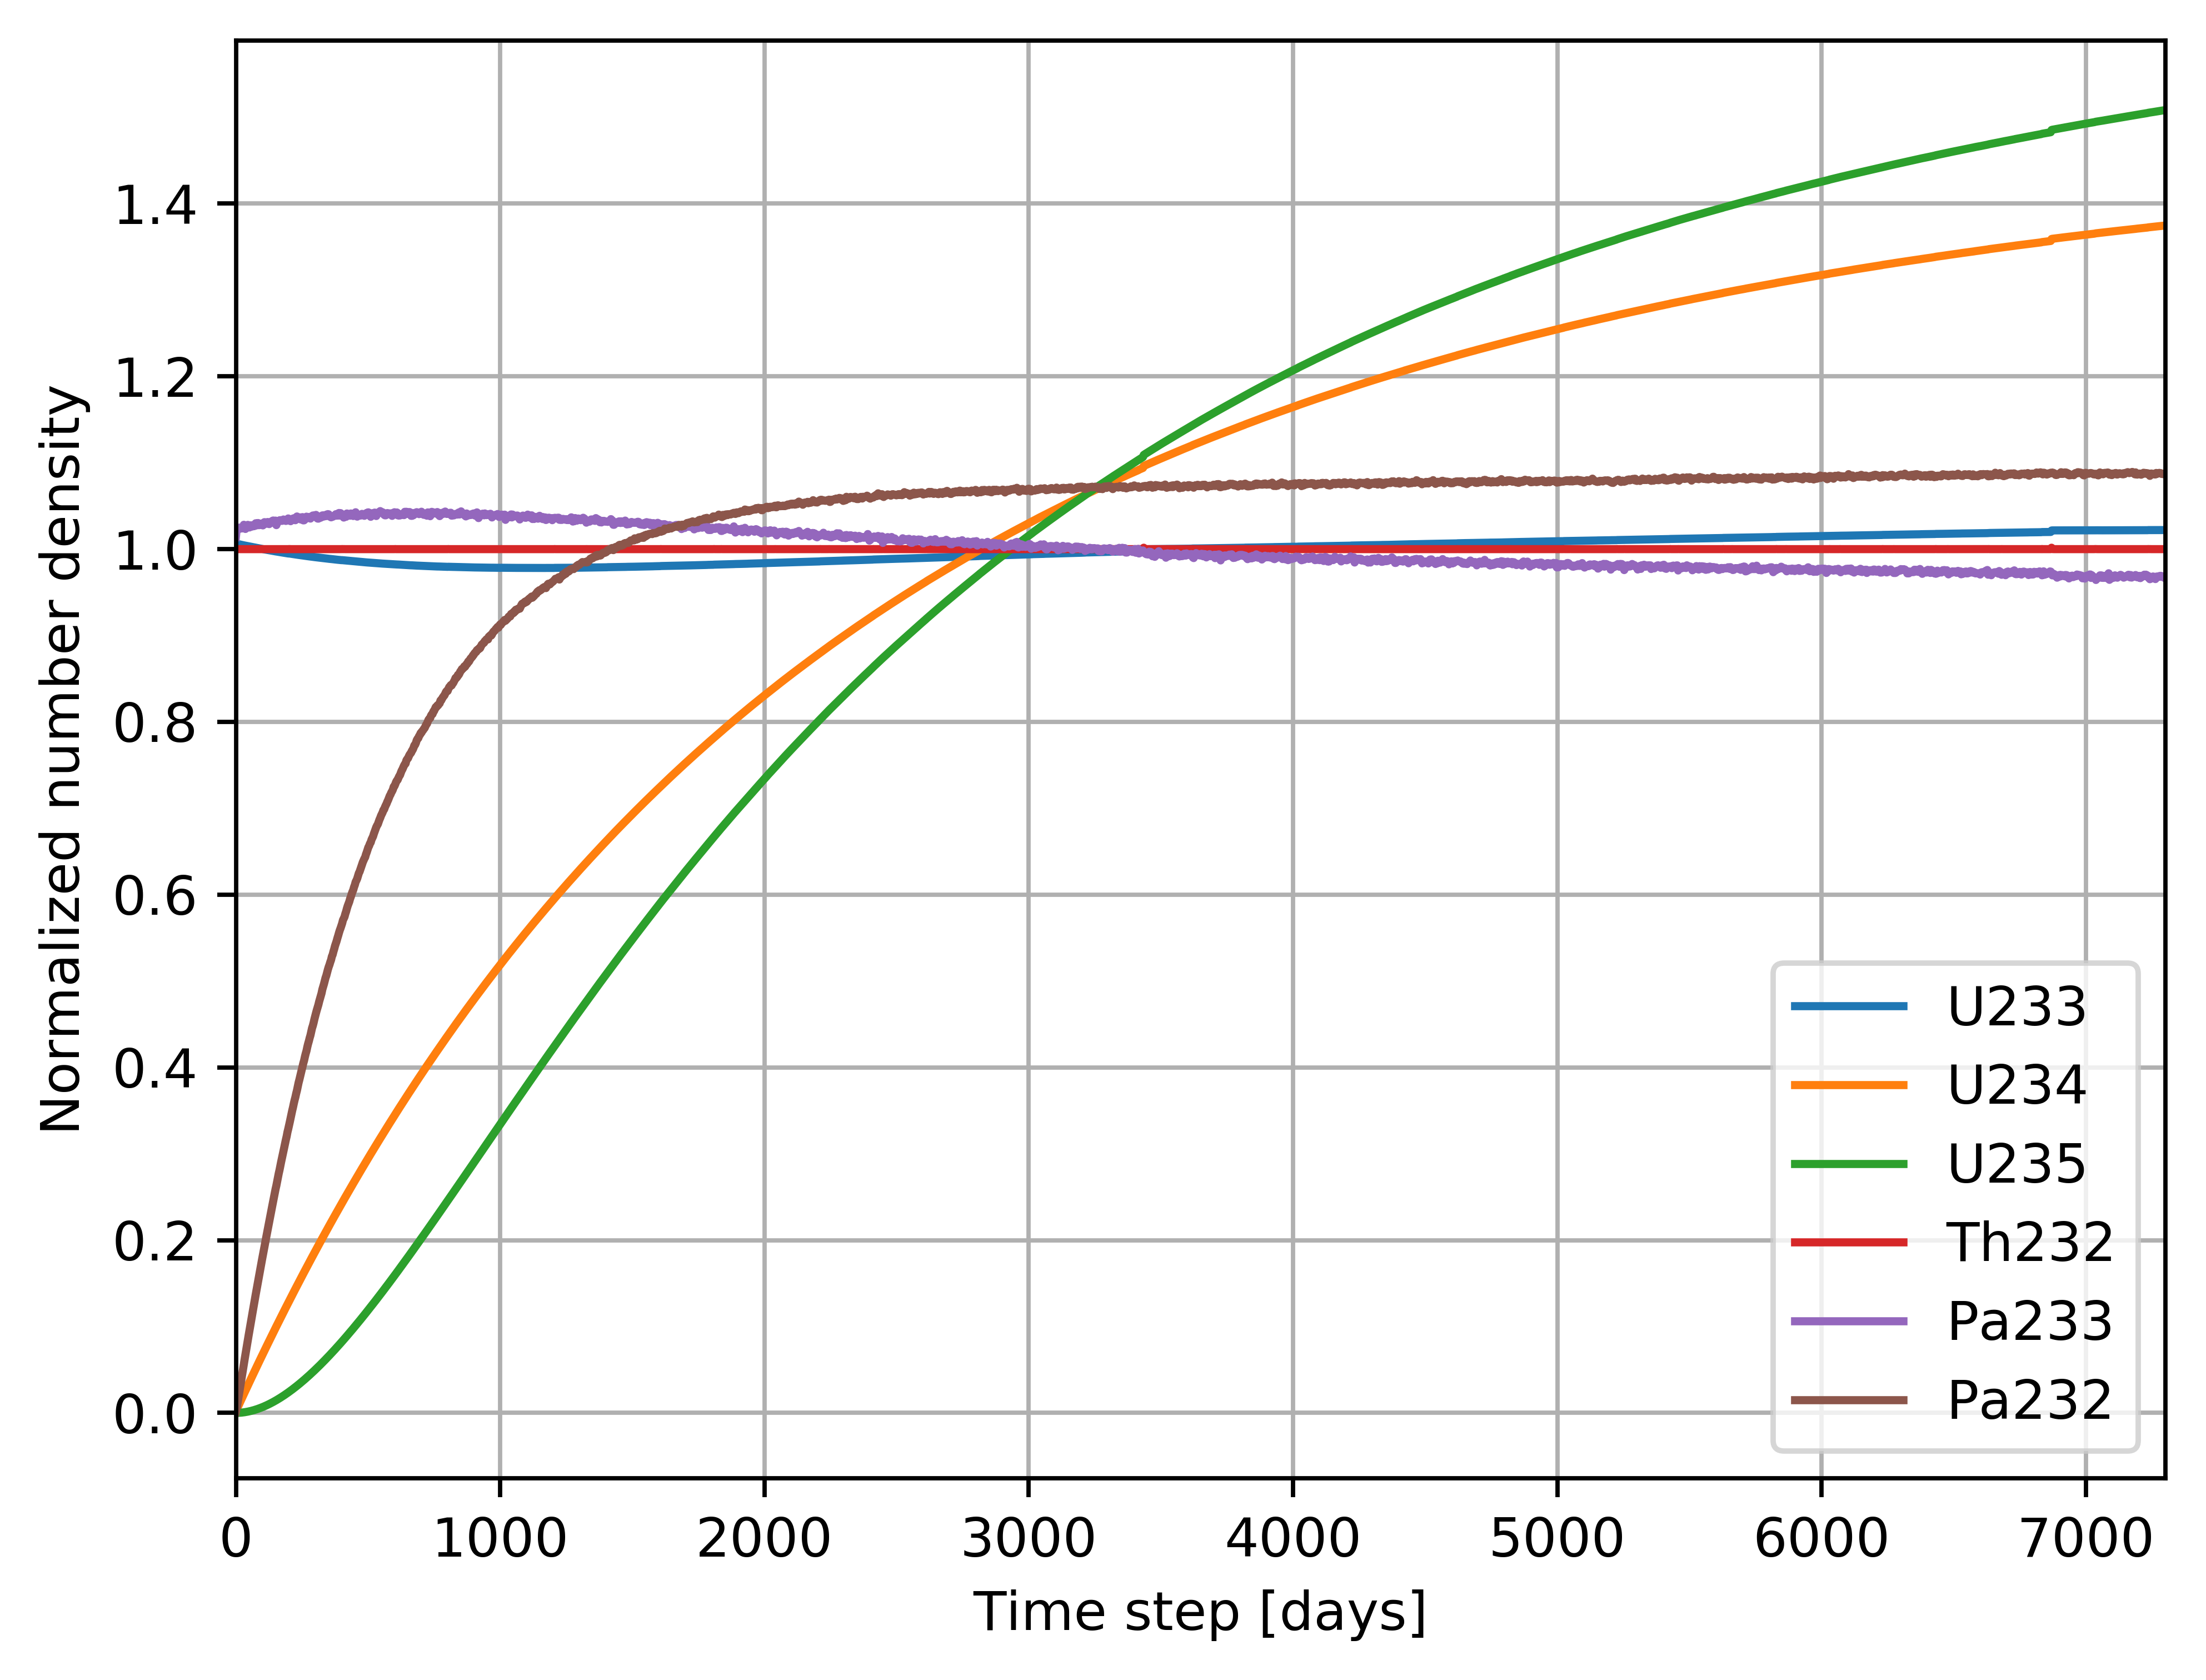
\includegraphics[width=1.05\textwidth]{major_isotopes_adens.png}
  \caption{Normalized number density of major nuclides during the reactor operation.}
  \vspace{-0.6em}
  \label{fig:adens_eq}
\end{figure}
\FloatBarrier

\begin{figure}[htp!] % replace 't' with 'b' to 
  \centering
  \vspace{-0.3em}
  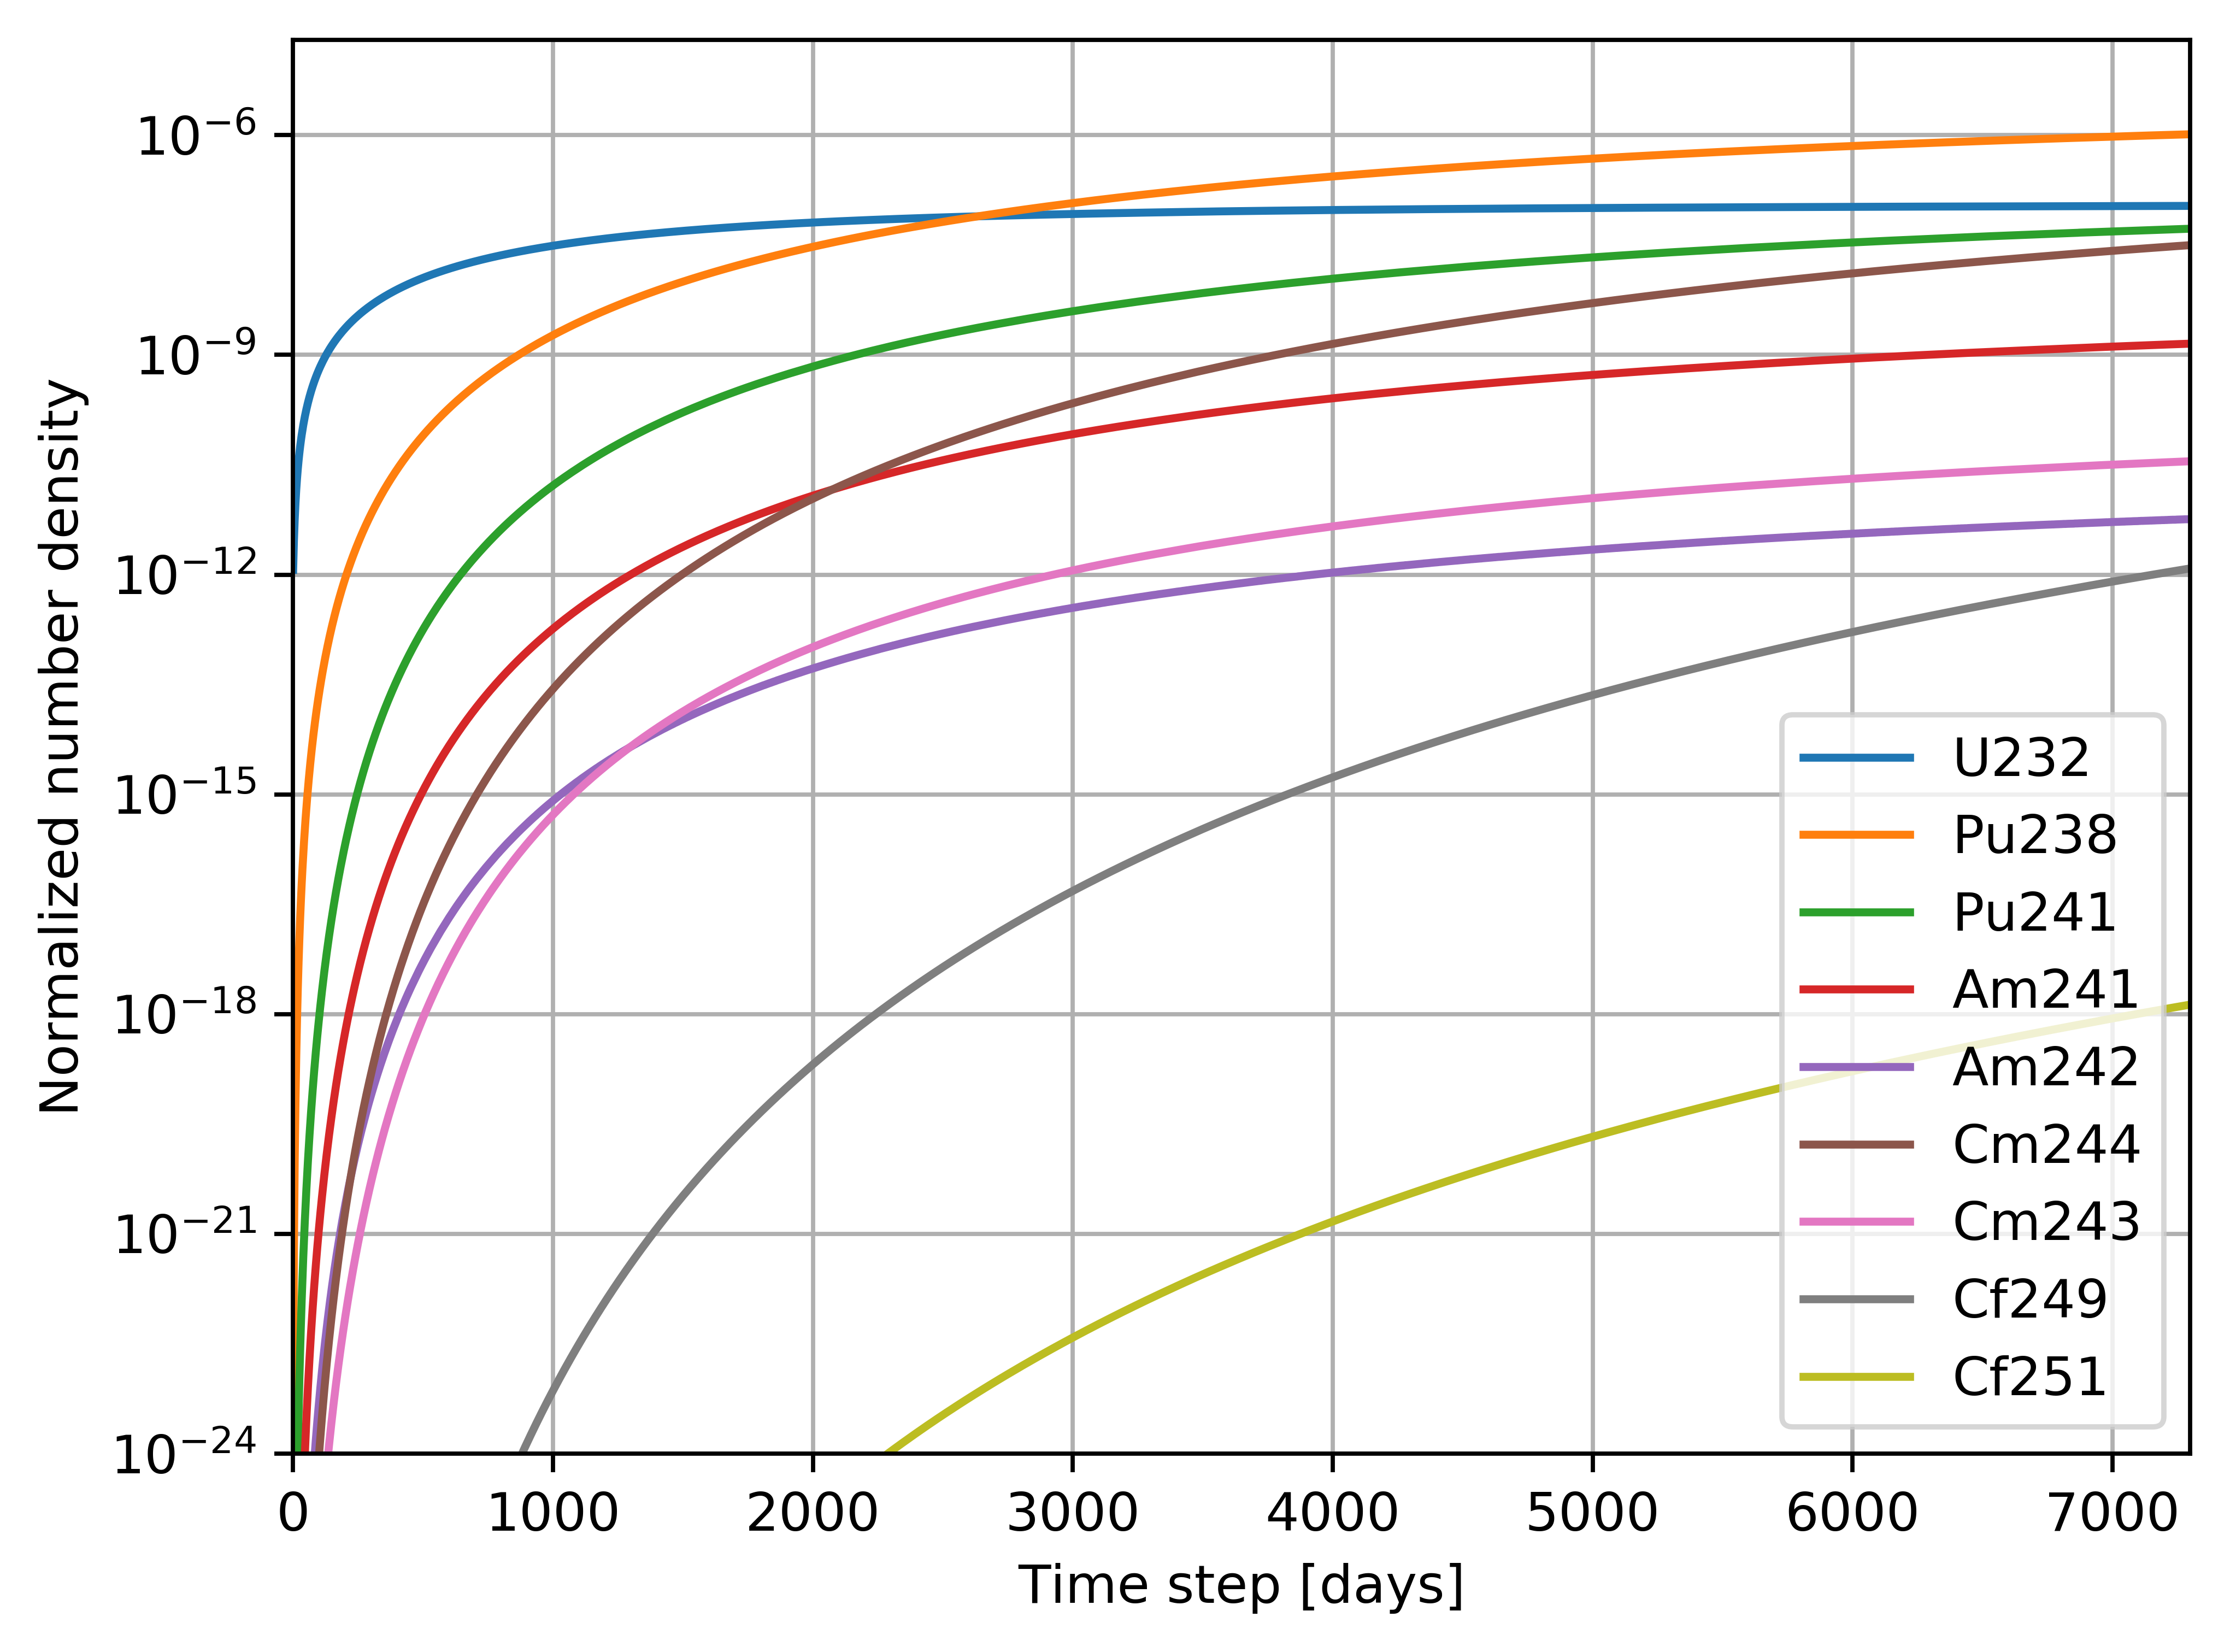
\includegraphics[width=1.05\textwidth]{fissile_short.png}
  \caption{Absolute number density of short-lived fissile nuclides (half live less than 900 years) during the reactor operation.}
  \vspace{-0.6em}
  \label{fig:fissile_short}
\end{figure}

\begin{figure}[hbp!] % replace 't' with 'b' to 
  \centering
  \vspace{-0.3em}
  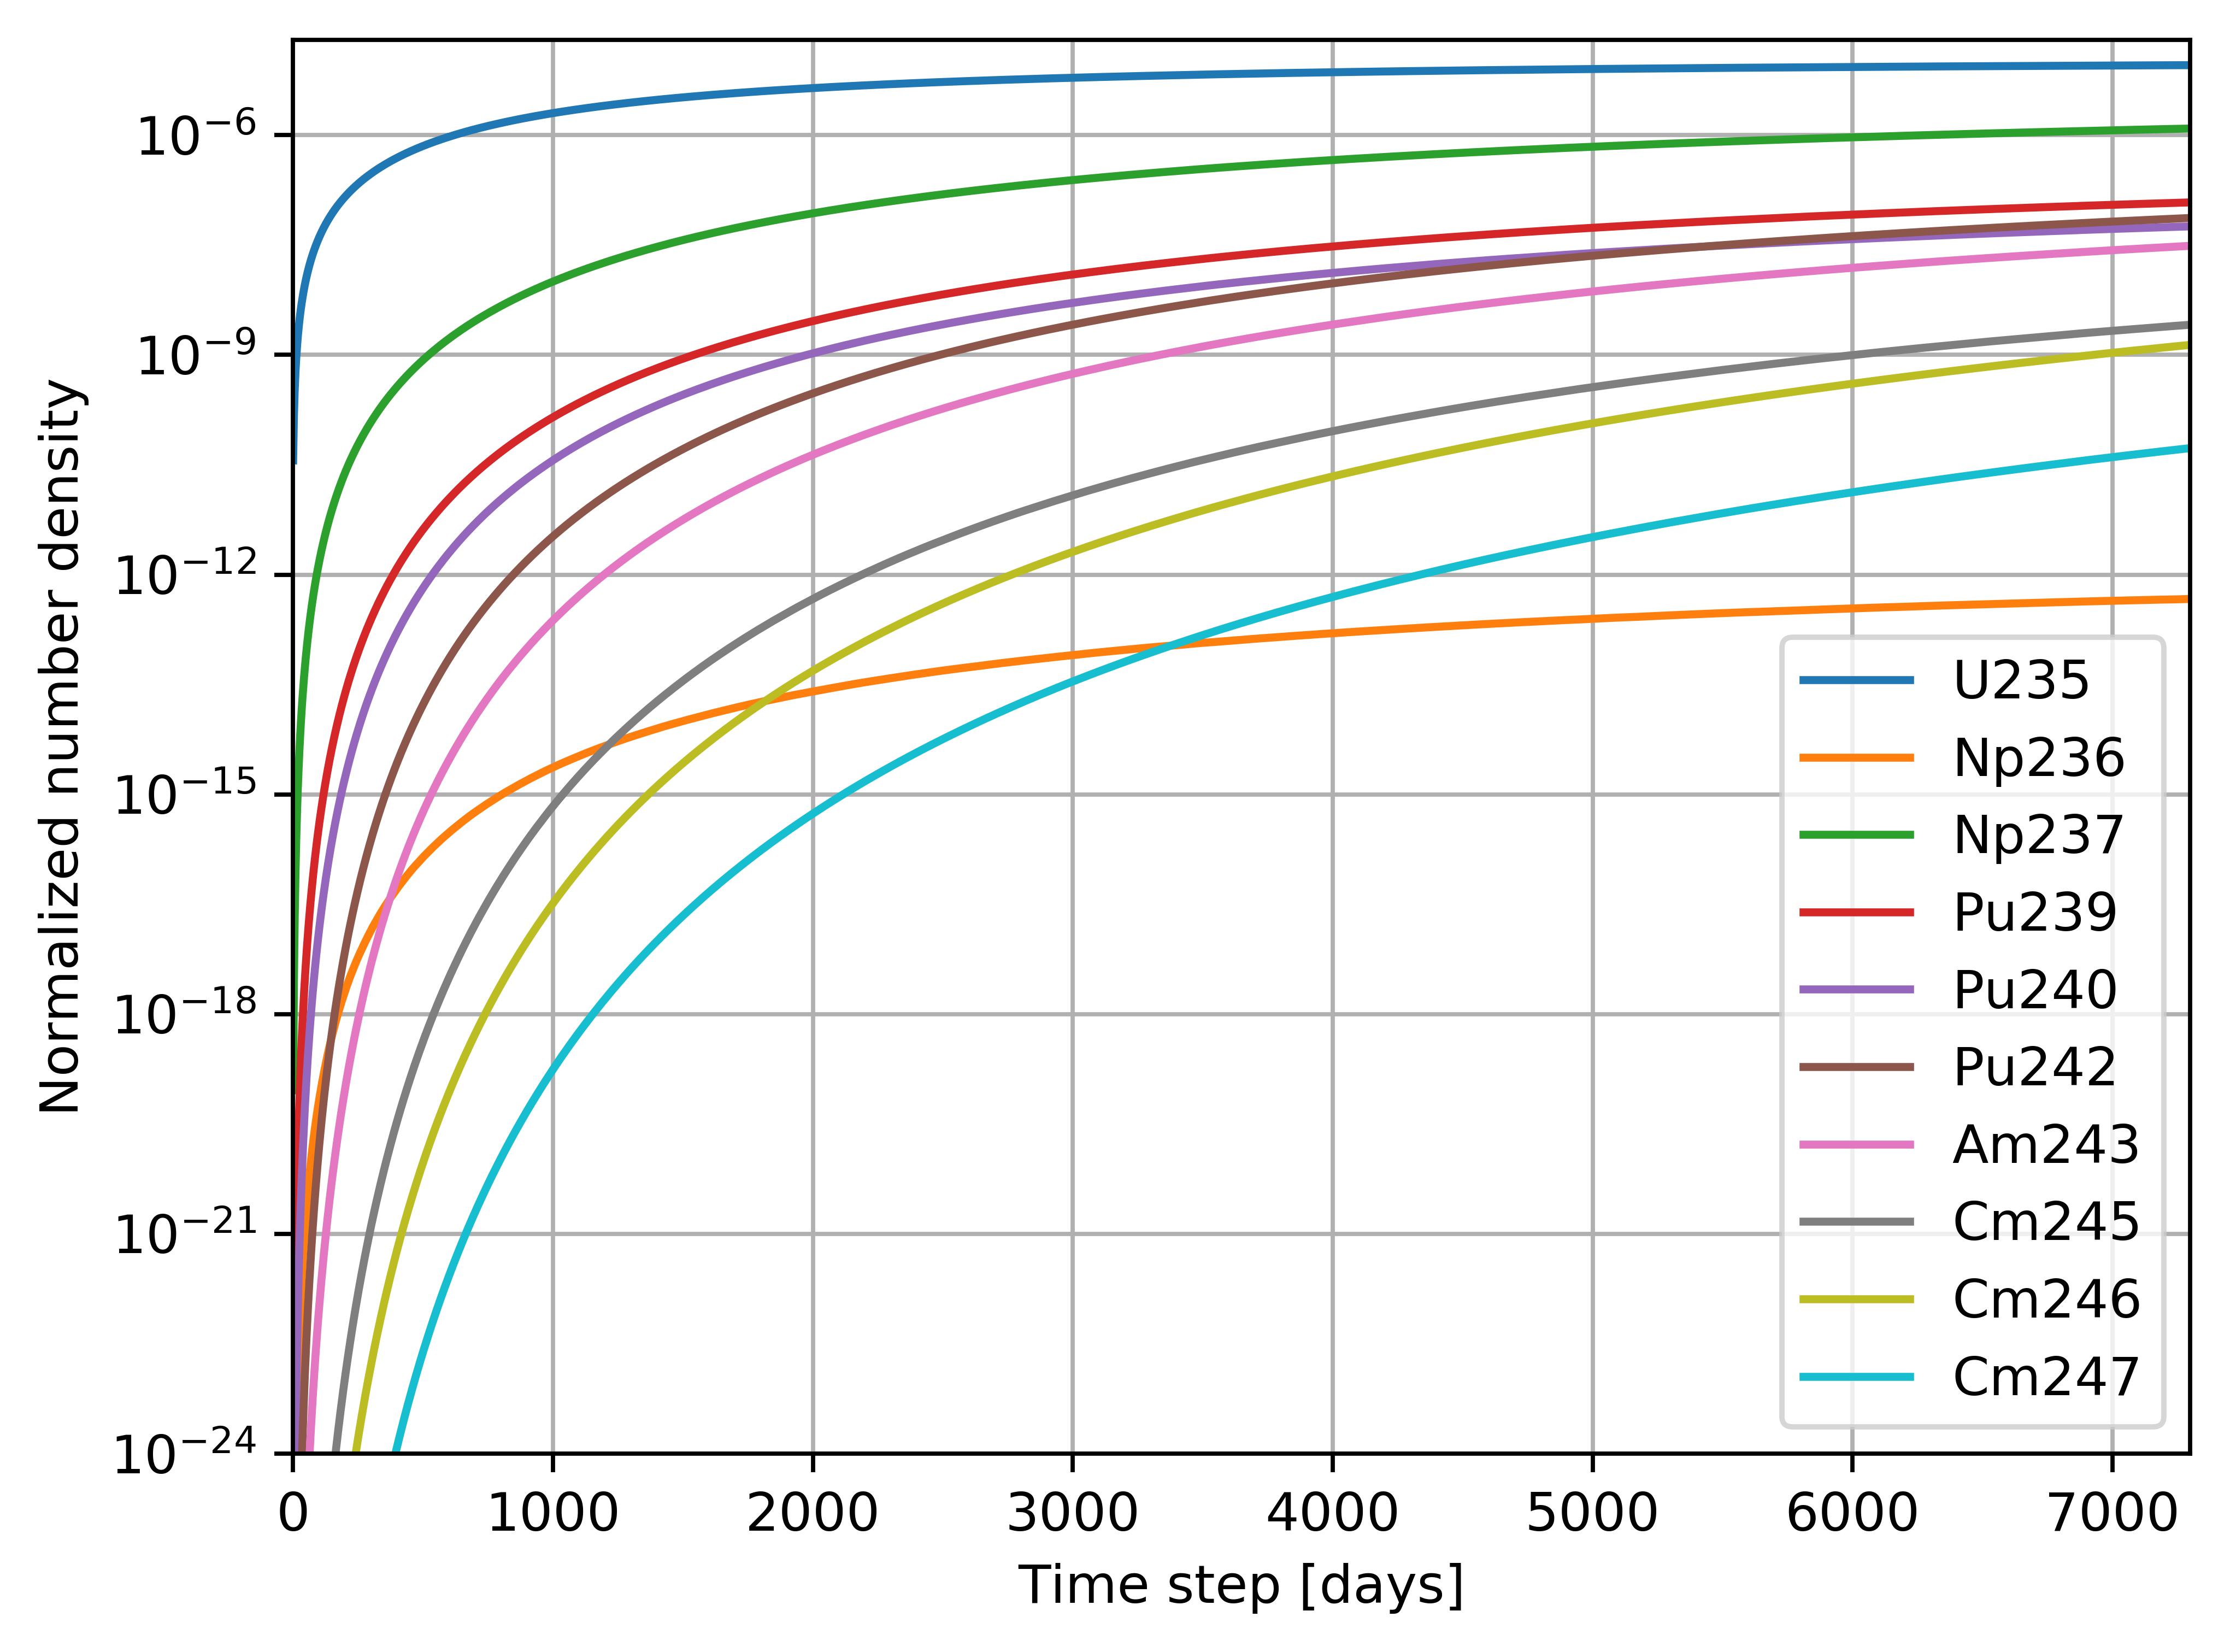
\includegraphics[width=1.05\textwidth]{fissile_long.png}
  \caption{Absolute number density of long-lived fissile nuclides (half live more than 900 years) during the reactor operation.}
  \vspace{-0.6em}
  \label{fig:fissile_long}
\end{figure}
\FloatBarrier

\section{Neutron spectrum}
Figure~\ref{fig:spectrum} demonstrates the normalized neutron flux spectrum for the full-core \gls{MSBR} model in the energy range from $10^{-8}$ to $10$ MeV. Neutron energy spectrum for equilibrium composition for the full-core is harder than for initial fuel loading due to $^{238}$Pu, $^{239}$Pu, $^{240}$Pu, $^{241}$Pu, $^{242}$Pu accumulation in the core during reactor operation. 

\begin{figure}[htp!] % replace 't' with 'b' to force it to 
  \centering
    \vspace{-0.3em}
  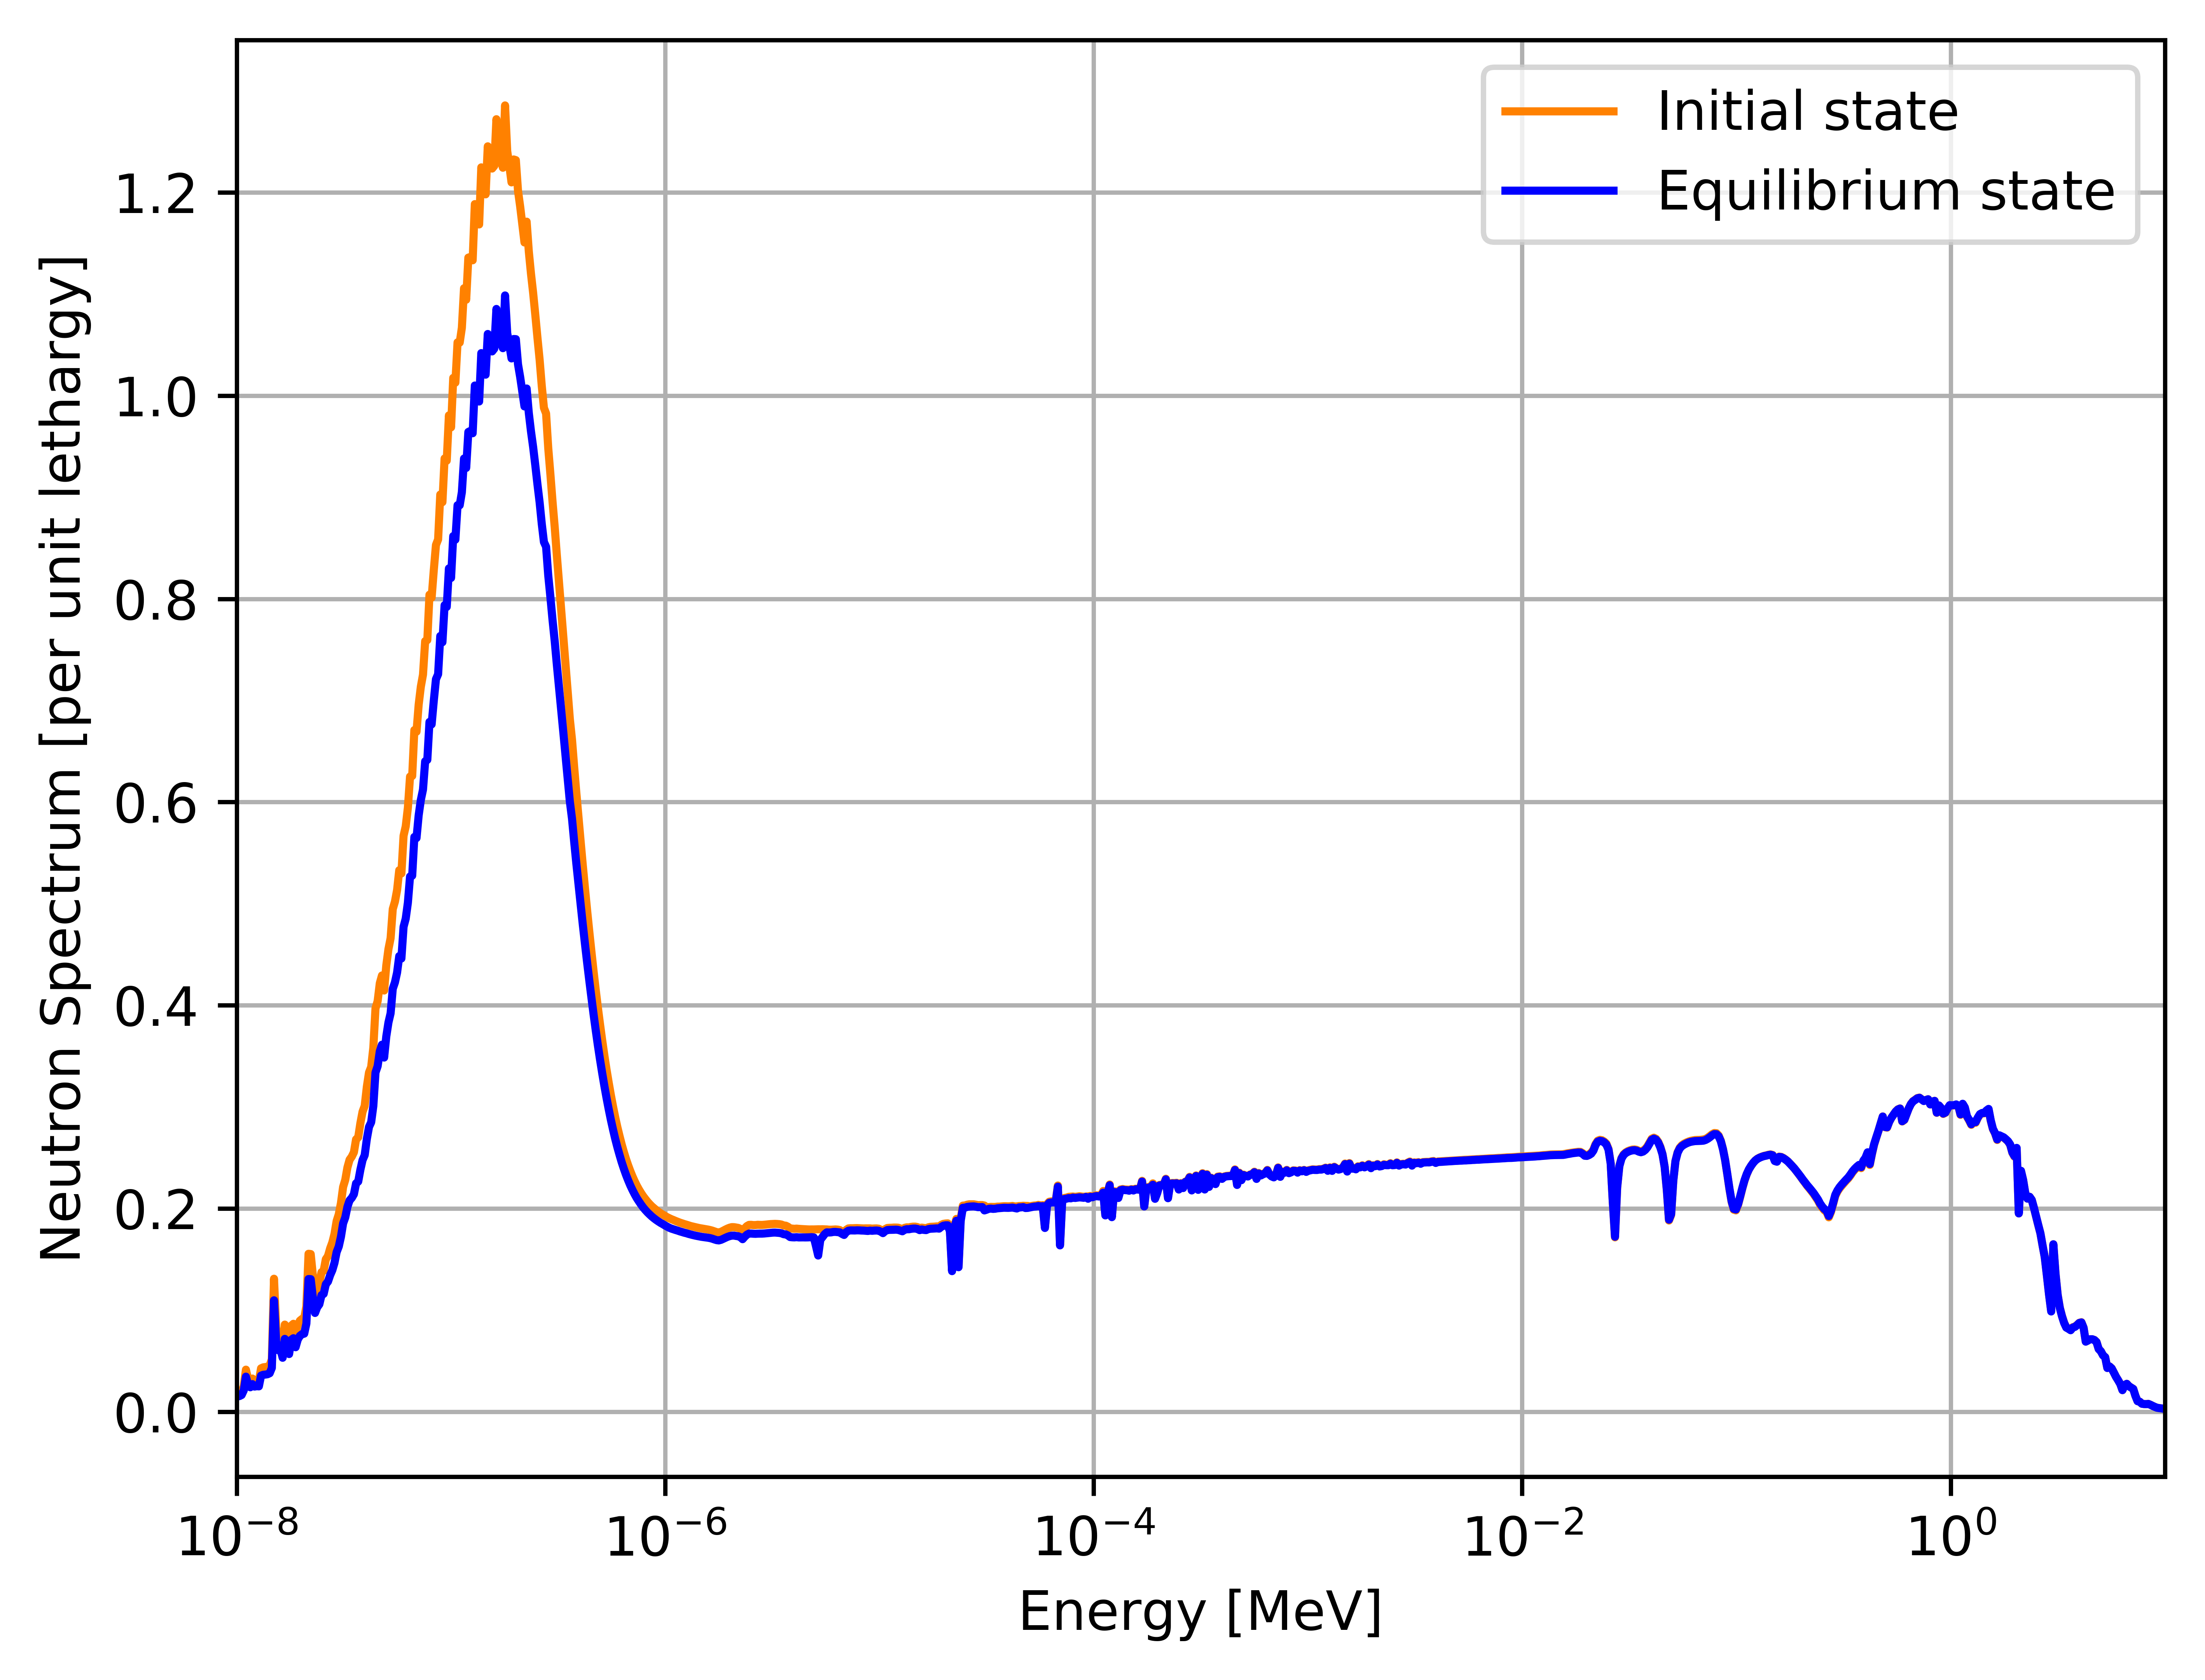
\includegraphics[width=1.05\textwidth]{spectrum.png} 
  \caption{Neutron flux energy spectrum normalized by unit lethargy for initial and equilibrium fuel salt composition.}
    \vspace{-0.6em}
  \label{fig:spectrum}
\end{figure}
\FloatBarrier

Figure~\ref{fig:spectrum_zones} shows that zone I produced much more thermal neutrons than zone II, consequently, the major number of fissions occurs in the central part of the core. In undermoderated zone II neutron energy spectrum is harder which leads to more capture of neutrons by $^{232}$Th and helps achieve relatively high breeding ratio. Moreover, resonances energy range for (n,$\gamma$) reaction for $^{232}$Th is from 10$^{-4}$ to 10$^{-2}$ MeV, therefore, moderator-to-fuel ratio for zone II was chosen to shift neutron energy spectrum in this range. Indeed, in the central core region (zone I) neutron energy spectrum was significantly shifted to harder spectrum over 20 years of fuel salt irradiation. In contrast, in the outer core region (zone II) such spectral shift also taken place but in a much smaller scale. 

It is important to obtain the epithermal and thermal spectrum to produce $^{233}$U from $^{232}$Th because radiative capture cross section of thorium monotonically decreases from $10^{-10}$ MeV to $10^{-5}$ MeV. Hardening the spectrum tends to significantly increase resonance absorption in thorium and decrease the absorptions in fissile and construction materials. Thus, a signficant amount fissile material will be needed to make the reactor critical. 

\begin{figure}[htp!] % replace 't' with 'b' to force it to 
  \centering
    \vspace{-0.3em}
  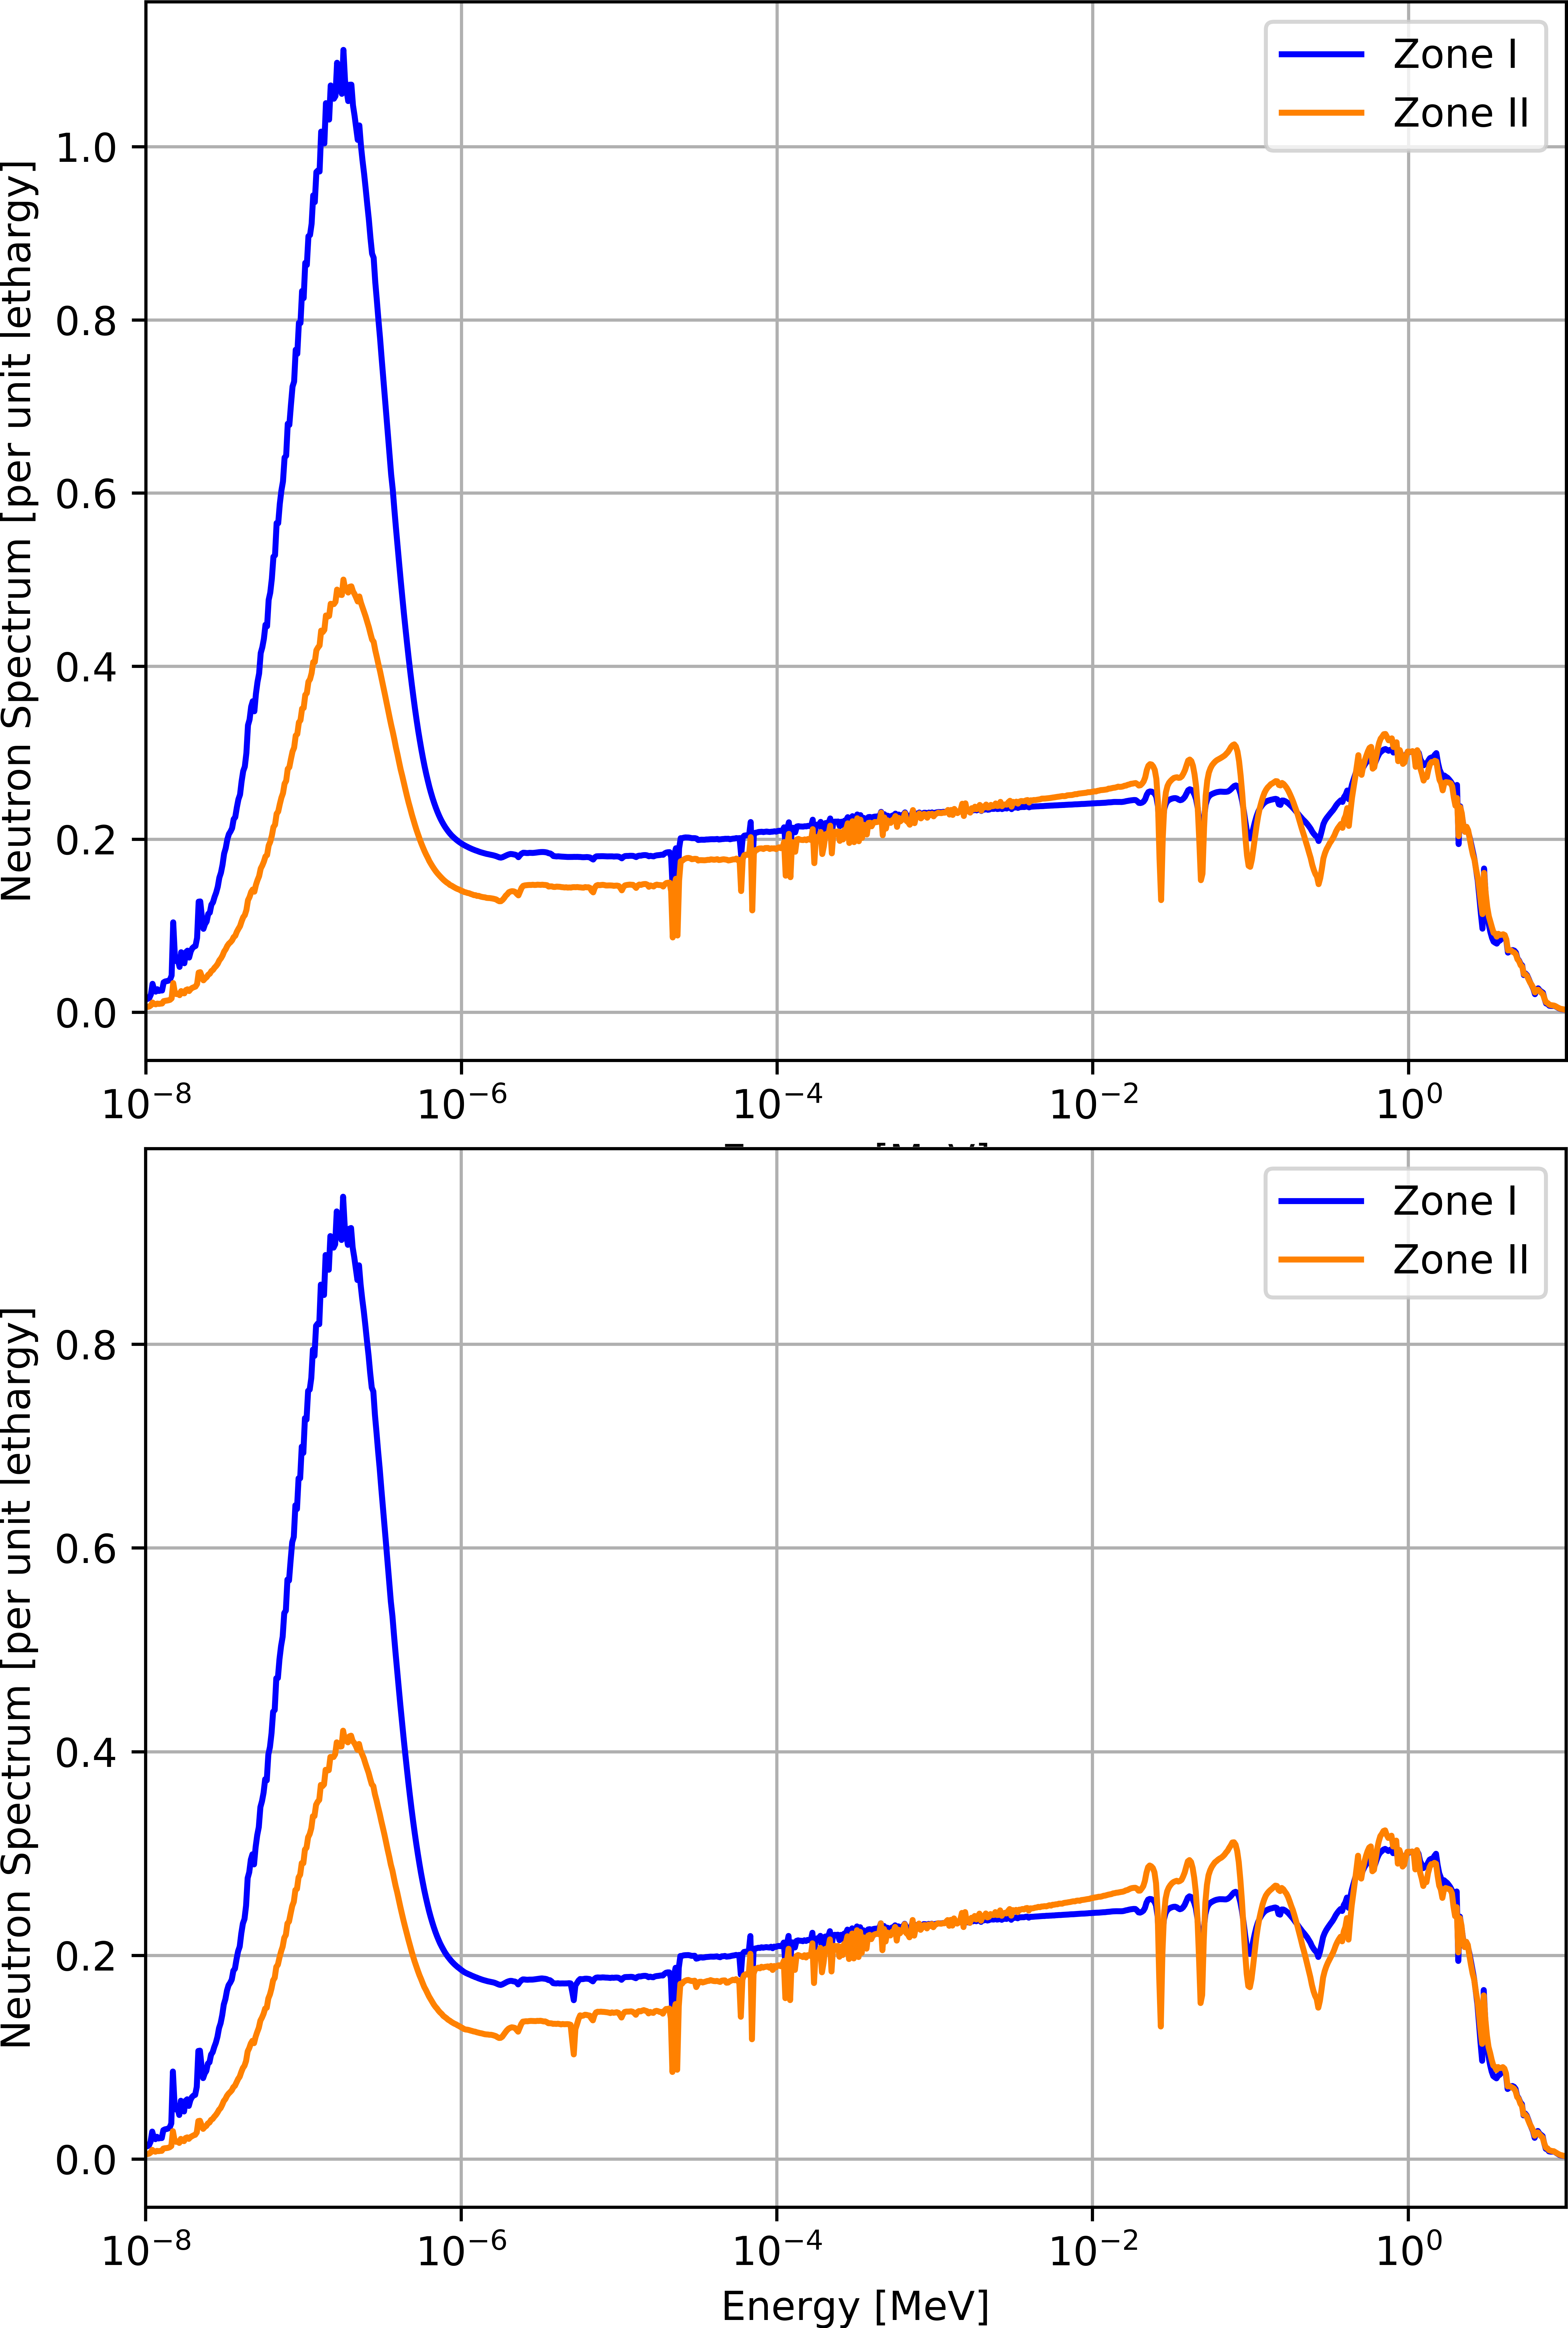
\includegraphics[width=\textwidth]{spectrum_by_zones.png} 
  \caption{Neutron flux energy spectrum in different core regions normalized by unit lethargy for initial (top) and equilibrium (bottom) fuel salt composition.}
    \vspace{-0.6em}
  \label{fig:spectrum_zones}
\end{figure}
\FloatBarrier

\section{Neutron flux}
Figure~\ref{fig:radial_flux} demonstrates radial distribution of fast and thermal neutron flux for both initial and equilibrium composition. Neutron flux has the same shape for both compositions but equilibrium case has harder spectrum. The significant spectral shift was observed for the central region of the core (for r from 0 to 200 cm) when for the outer region it is neglectable for fast but notable for thermal neutrons. On the whole, spectrum hardening during \gls{MSBR} operation should be carefully studied for designing reactivity control system.

\begin{figure}[htp!] % replace 't' with 'b' to force it to 
  \centering
    \vspace{-0.3em}
  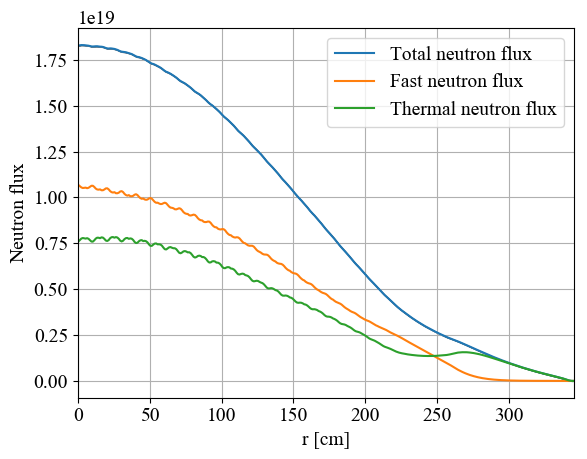
\includegraphics[width=1.05\textwidth]{radial_flux.png} 
  \caption{Radial neutron flux distribution for initial and equilibrium fuel salt composition.}
    \vspace{-0.6em}
  \label{fig:radial_flux}
\end{figure}
\FloatBarrier

\section{Power and breeding distribution}
Figure~\ref{fig:pow_den} demonstrates the normalized power distribution of the \gls{MSBR} one-fourth core at initial and equilibrium state.  For both the initial and equilibrium composition most of fission occurs in the center of the core, namely zone I. Similarly, major amount of gamma radiation heat, generated in reactor graphite due to neutron scattering and absorption, was released in zone I. Table~\ref{tab:powgen_fraction} shows the power fraction in each zone for the similar conditions. The spectral shift during the reactor operation results in different power fractions between the initial and equilibrium compositions but the most of power is still generated in zone I. Figure~\ref{fig:breeding_den} shows neutron capture reaction rate distribution for $^{232}$Th normalized by total neutron flux for initial and equilibrium state. The distribution demonstrates spatial distribution of $^{233}$Th production in the core. The thorium-232 then $\beta$-decaying to $^{233}$Pa which is precursor for $^{233}$U production, consequently, this distribution might be considered as breeding distribution in the \gls{MSBR} core. As could be seen from figures, spectral shift does not cause significant changes neither in power nor breeding distribution. Even after 20 years of irradiation, most of the heat power still generated in zone I when the major amount of $^{233}$Th produced in zone II.

%%%%%%%%%%%%%%%%%%%%%%%%%%%%%%%%%%%%%%%%
\begin{table}[ht!]
  \centering
  \caption{Power generation fraction in each zone for initial and equilibrium state.}
\begin{tabular}{| m{0.22\textwidth} | m{0.22\textwidth} | m{0.22\textwidth} |} \hline
Core region      & Initial      & Equilibrium   \\ [3pt]\hline   
Zone I           & 97.91\%      & 98.12\%   \\ [3pt] \hline
Zone II          & 2.09\%       & 1.88\%   \\ [3pt] \hline
\end{tabular}
  \label{tab:powgen_fraction}
\end{table}
%%%%%%%%%%%%%%%%%%%%%%%%%%%%%%%%%%%%%%%%%%%%%%%%%%%%%%%%%%%%%%%%%%%%%%%%%%%%%%%%

\begin{figure}[htp!] % replace 't' with 'b' to force it to 
  \centering
    \vspace{-0.3em}
  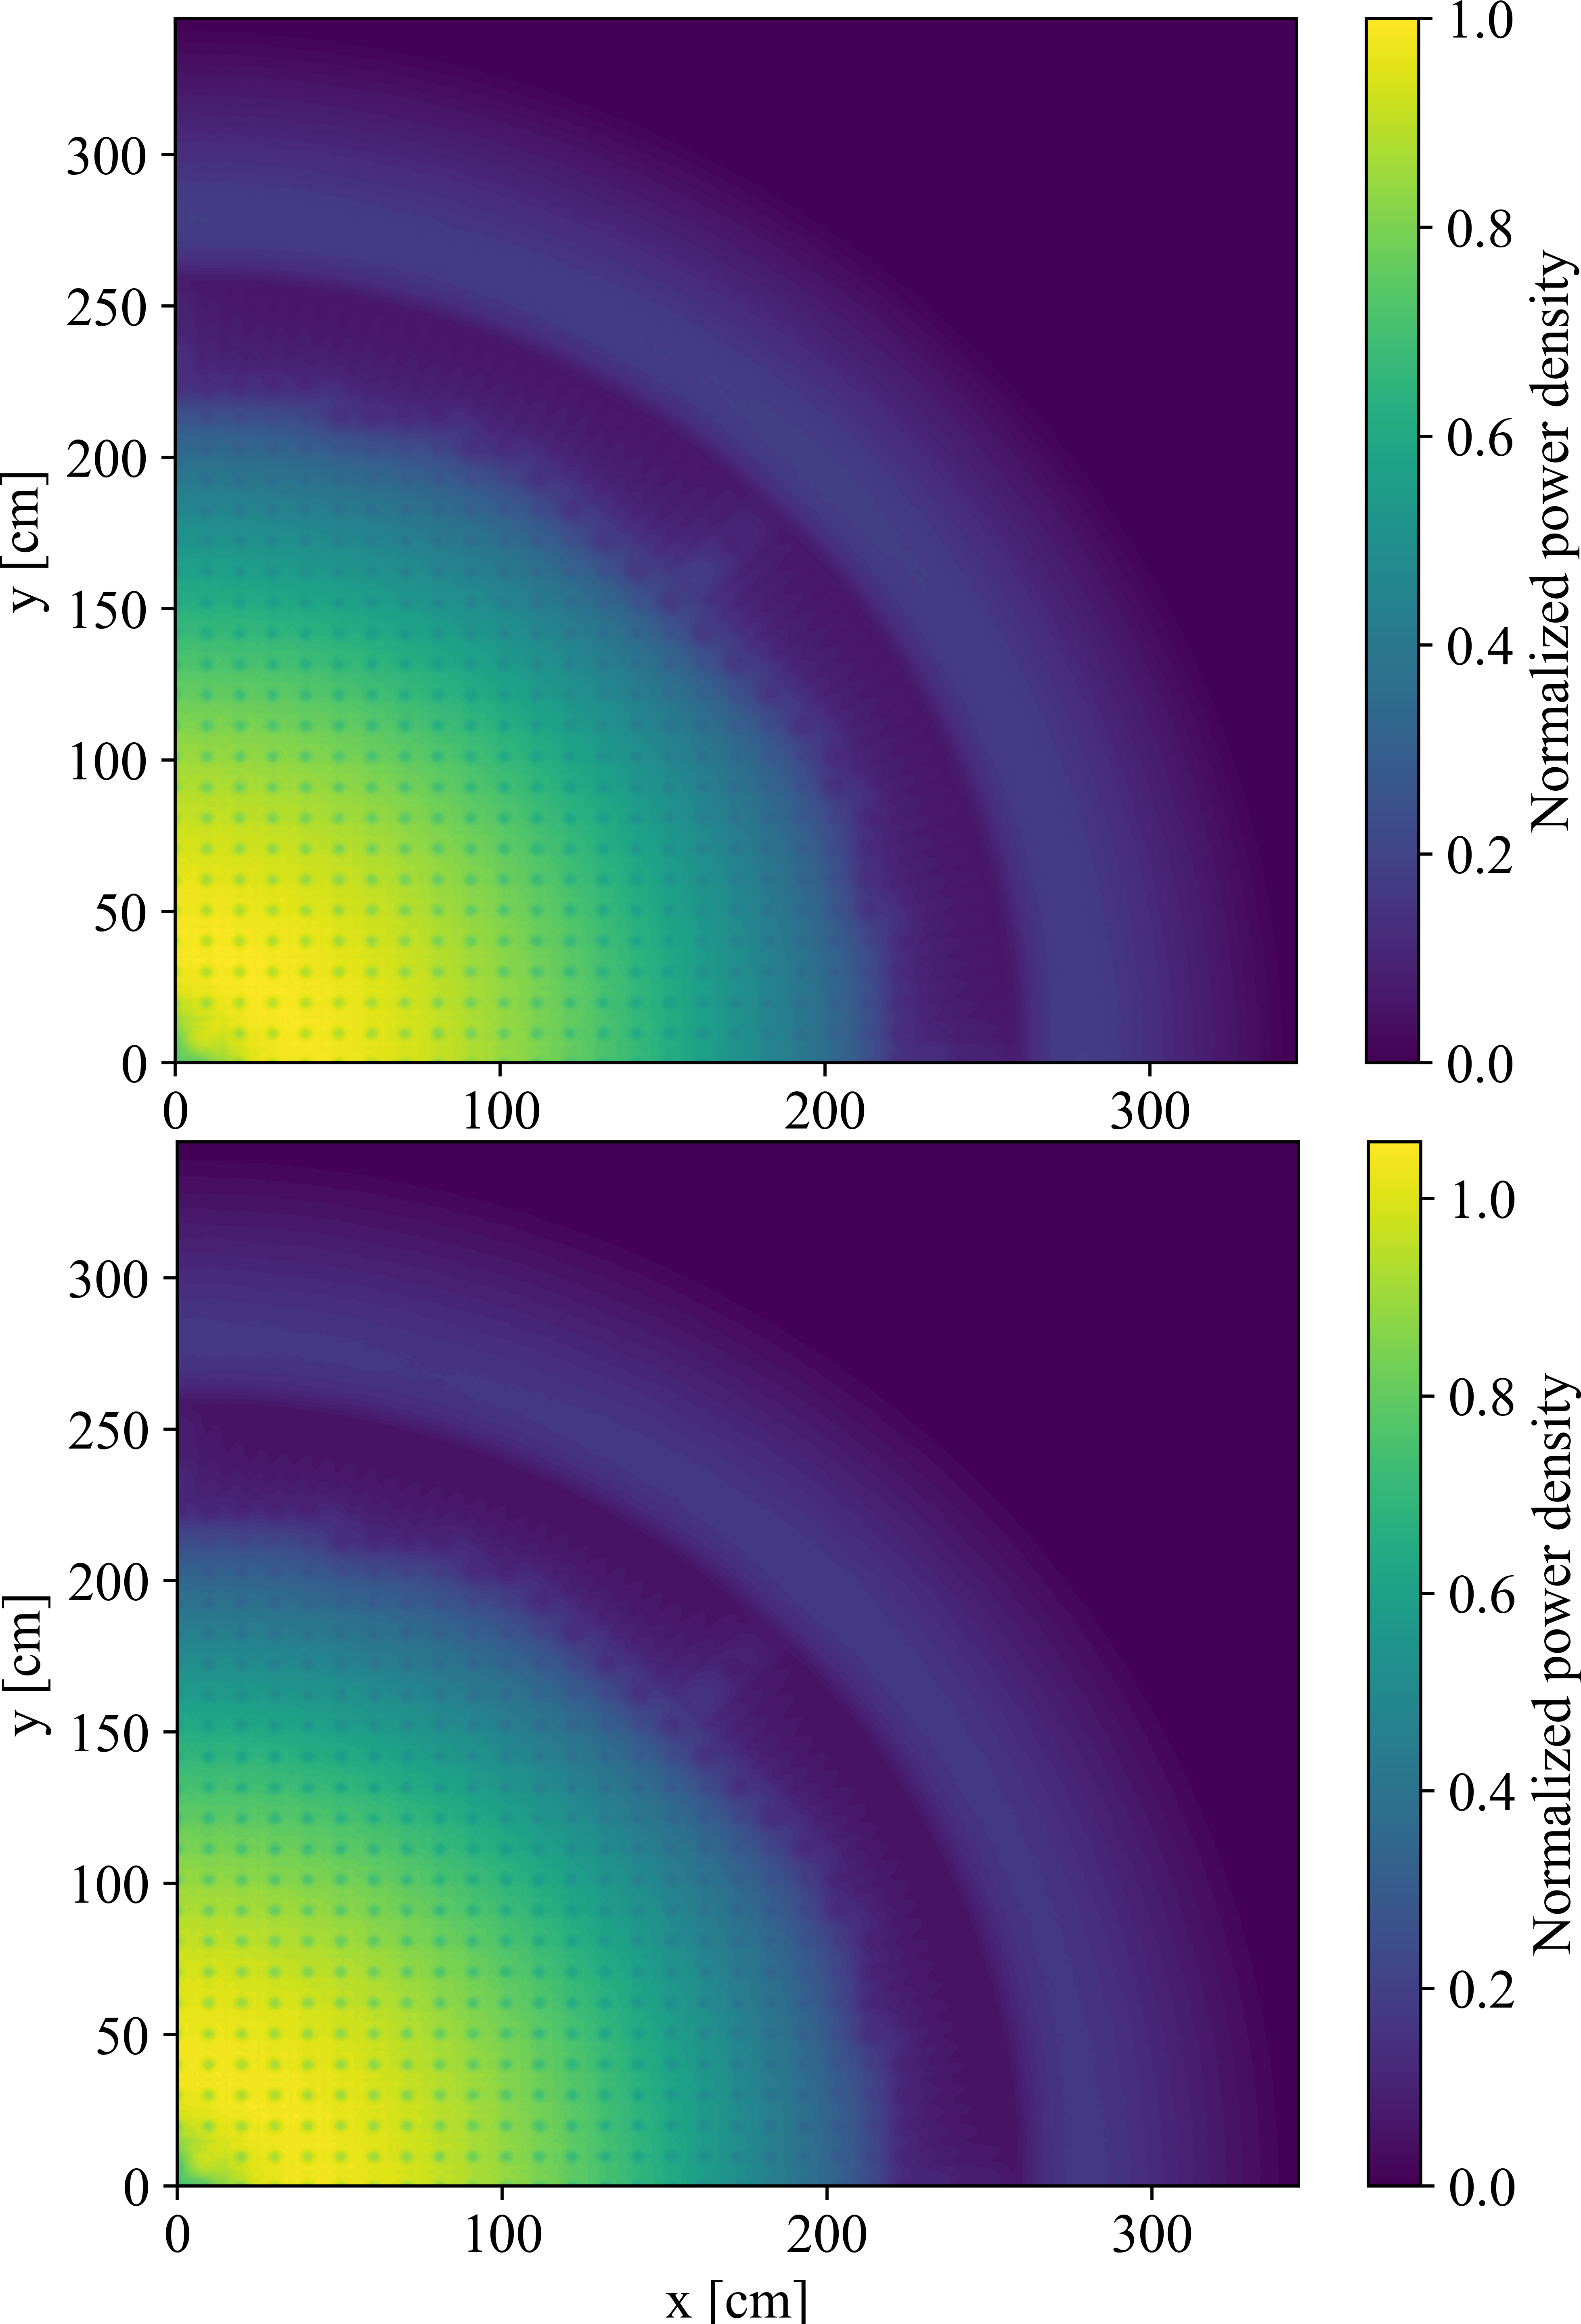
\includegraphics[width=1.05\textwidth]{power_distribution.png} 
  \caption{Normalized power density for initial (top) and equilibrium (bottom) fuel salt composition.}
    \vspace{-0.6em}
  \label{fig:pow_den}
\end{figure}
\FloatBarrier

\begin{figure}[htp!] % replace 't' with 'b' to force it to 
  \centering
    \vspace{-0.3em}
  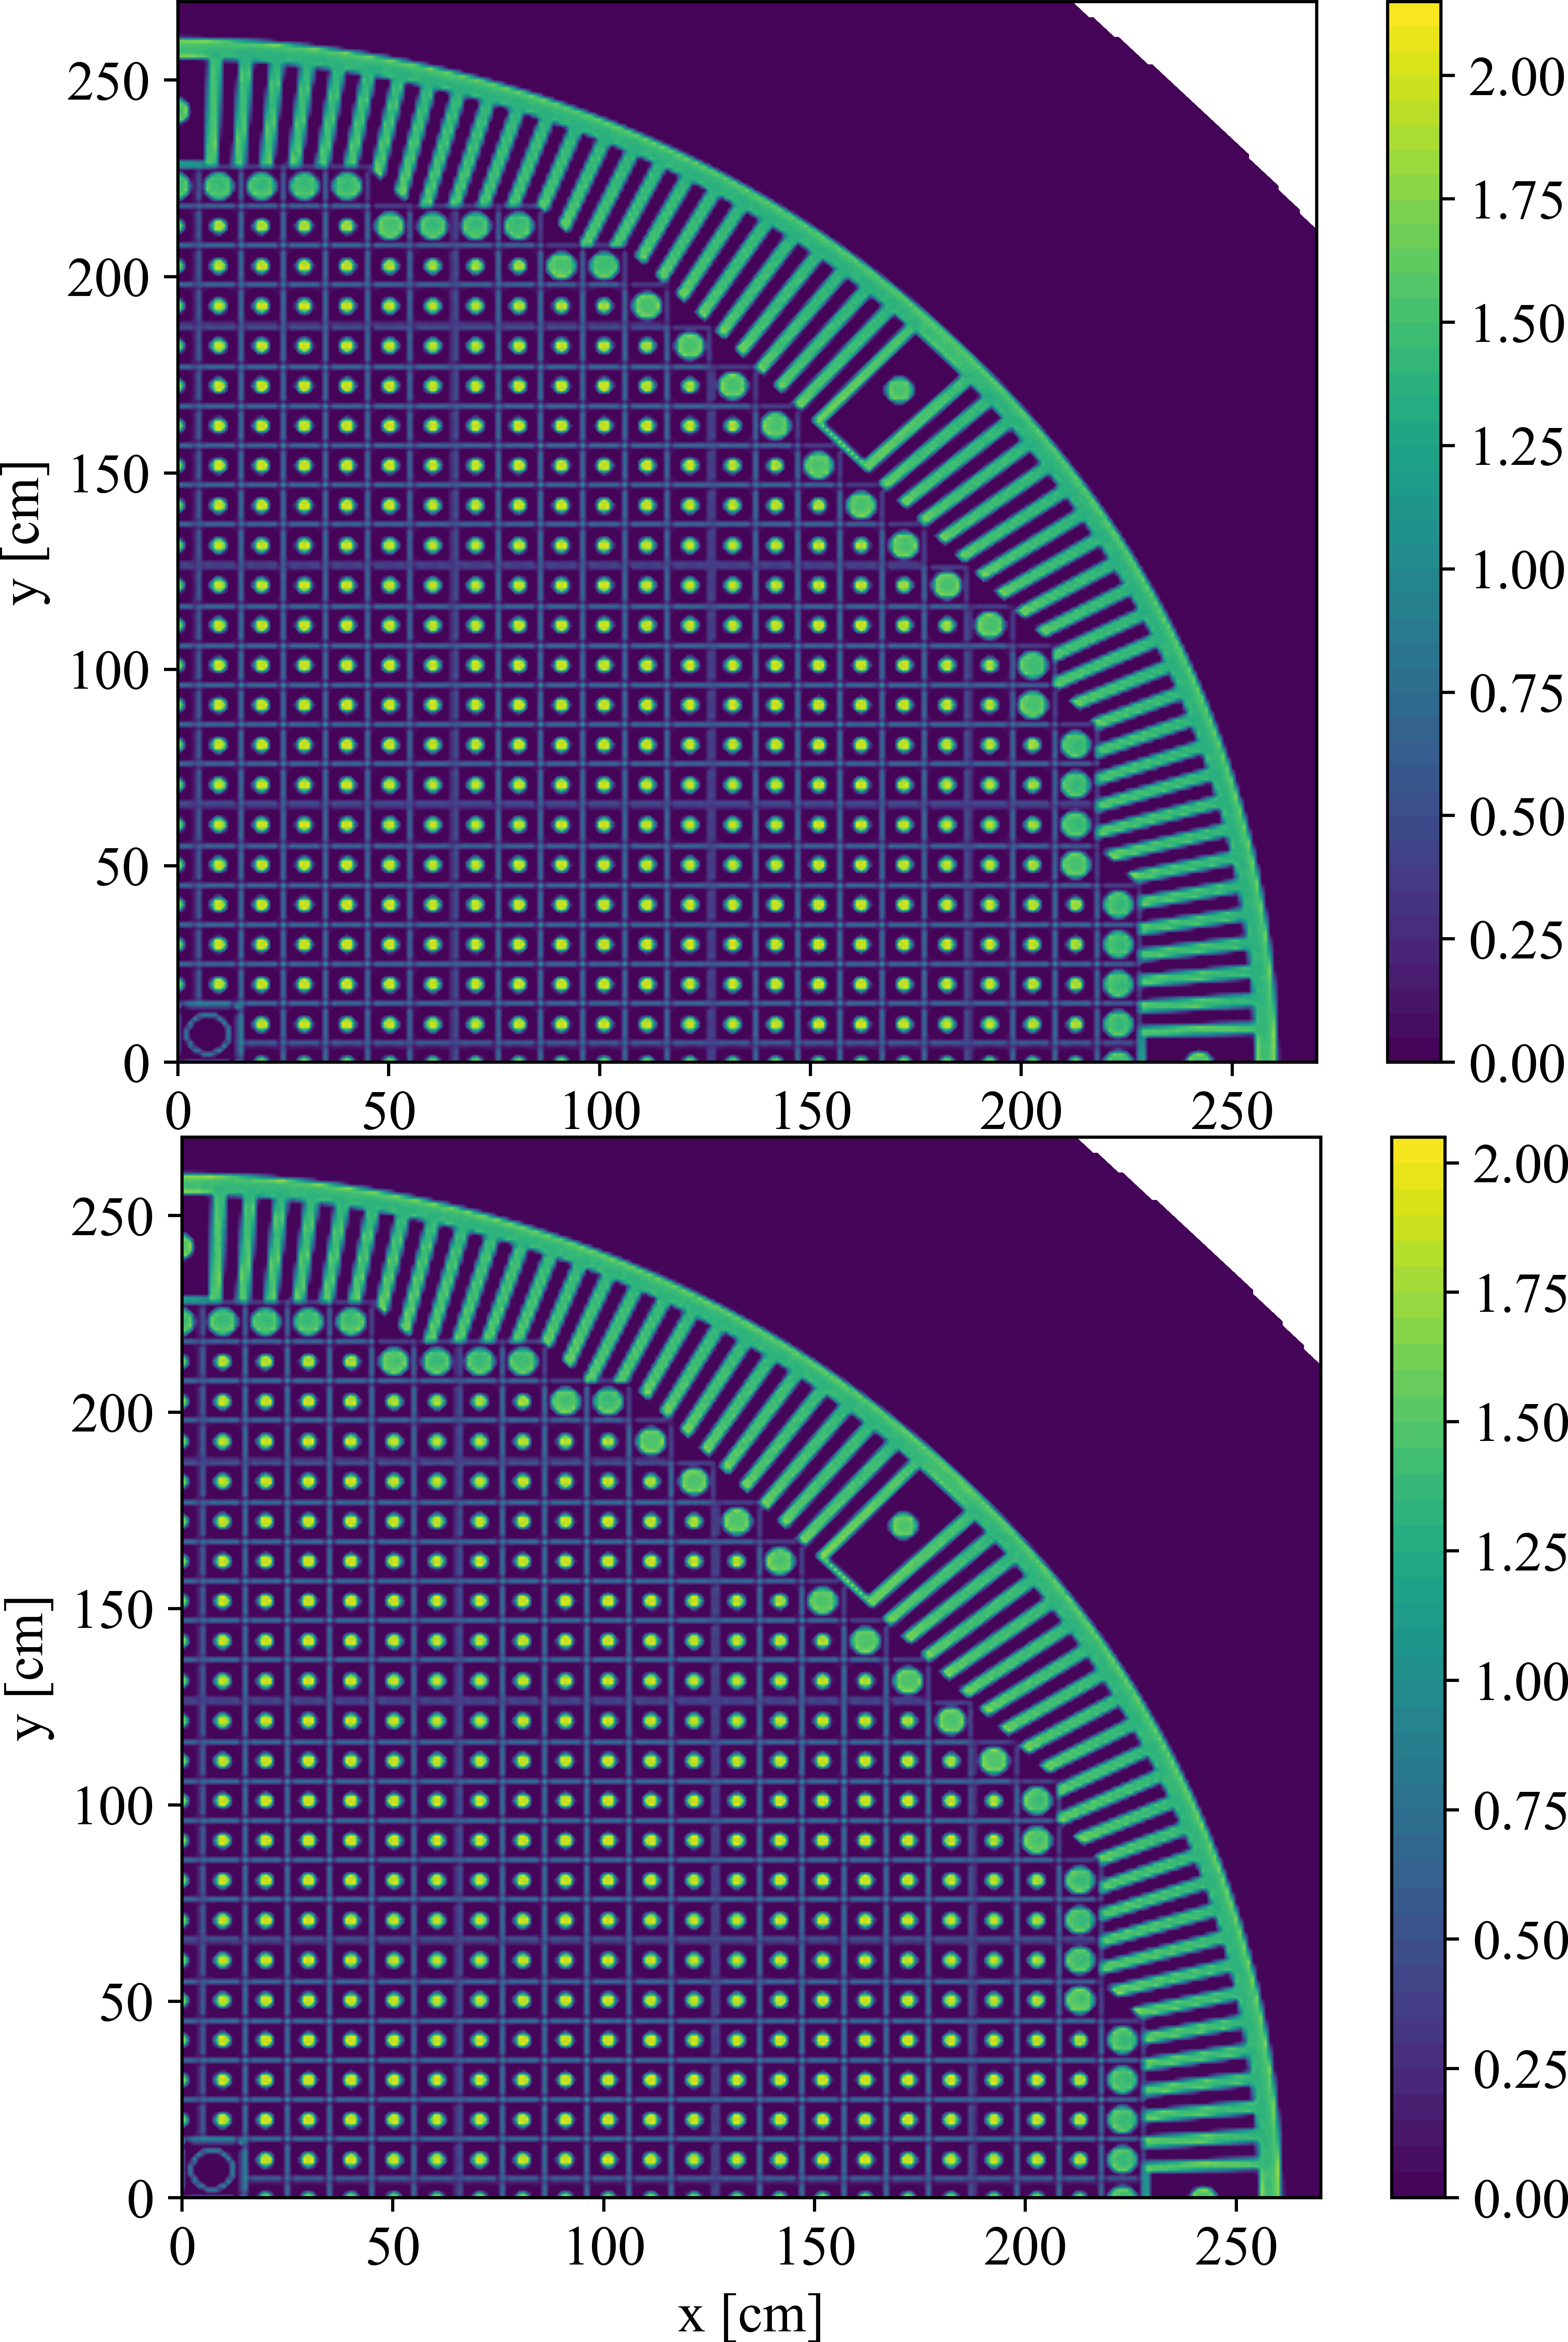
\includegraphics[width=1.05\textwidth]{breeding_distribution.png} 
  \caption{$^{232}$Th neutron capture reaction rate normalized by total flux for initial (top) and equilibrium (bottom) fuel salt composition.}
    \vspace{-0.6em}
  \label{fig:breeding_den}
\end{figure}
\FloatBarrier

\section{Temperature effect of reactivity}
Table~\ref{tab:tcoef} summarizes temperature effects on reactivity calculated in this work for both initial, equilibrium fuel composition and compared with original \gls{ORNL} report data \cite{robertson_conceptual_1971}. Uncertainty for each temperature coefficient also appears in Table~\ref{tab:tcoef}. The main physical principle underlying the reactor temperature feedback is an expansion of matter when it is heated. When the fuel salt temperature increases, the density of the salt decreases, but at the same time, the total volume of fuel salt in the core remains 
constant because it is bounded by the graphite. When the reactor graphite temperature grows, the density of graphite declines creating additional space for fuel salt. To determine temperature coefficients, the cross-section temperatures for fuel and moderator were changed from 900K to 1000K. Three different cases were considered:
\begin{enumerate}
  \item Temperature of fuel salt rising from 900K to 1000K.
  \item Temperature of graphite rising from 900K to 1000K.
  \item Whole reactor temperature rising from 900K to 1000K.
\end{enumerate}

%%%%%%%%%%%%%%%%%%%%%%%%%%%%%%%%%%%%%%%%
\begin{table}[ht!]
  \centering
  \caption{Temperature coefficients of reactivity for initial and equilibrium state.}
\begin{tabular}{| m{0.22\textwidth} | m{0.22\textwidth} | m{0.22\textwidth} | m{0.22\textwidth} |} \hline
   Reactivity coefficient [pcm/K]  & Initial      & Equilibrium  & Reference \cite{robertson_conceptual_1971} \\ [5pt]\hline   
Fuel salt        & $-3.22\pm0.044$ & $-1.53\pm0.046$ & $-3.22$  \\ [3pt] \hline
Moderator        & $+1.61\pm0.044$ & $+0.97\pm0.046$ & $+2.35$  \\ [3pt] \hline
Total            & $-3.1\pm0.04$   & $-0.97\pm0.046$ & $-0.87$  \\ [3pt] \hline
\end{tabular}
  \label{tab:tcoef}
\end{table}
%%%%%%%%%%%%%%%%%%%%%%%%%%%%%%%%%%%%%%%%%%%%%%%%%%%%%%%%%%%%%%%%%%%%%%%%%%%%%%%%
In the first case, changes in the fuel temperature only impact fuel density. In this case, the geometry is unchanged because fuel is a liquid. However, when the moderator heats up, both the density and the geometry change due to thermal 
expansion of the solid graphite blocks and reflector. Accordingly, the new graphite density was calculated using a linear temperature expansion coefficient of 1.3$\times10^{-6}$1/K \cite{robertson_conceptual_1971}. A new geometry input was created based on this information.

The fuel temperature coefficient (FTC) is negative for both initial and equilibrium fuel compositon due to thermal Doppler broadening of the resonance capture cross sections in the thorium and is in a good agreement with early research \cite{robertson_conceptual_1971,park_whole_2015}. The moderator temperature coefficient (MTC) is positive for initial compositions due to changing density and decreasing during reactor operation because of spectrum hardening along with fuel depletion. Finally, the total temperature coefficient of reactivity is negative for both cases, but it is decreasing during reactor operation due to spectral shift the same as MTC. In sum, even after 20 years of irradiation the total temperature coefficient of reactivity is relatively large and negative during reactor operation, despite graphite components, and affords excellent reactor stability and controllability.

\section{Reactivity control system rod worth}
Table~\ref{tab:rod_worth} summarizes the reactivity control system efficiency calculation results. At the normal operation condition, the control (graphite) rods are fully inserted, and the safety (B$_4$C) rods are fully withdrawn. To insert negative reactivity into the core, the graphite rods are gradually withdrawn from the core. In an accident, the safety rods would fall down into the core. The rod integral worths were calculated for various positions to estimate separately control (graphite) rod, safety (B$_4$C) rod, and the whole reactivity control system worth. Control rod integral worth is about 28 cents and stay almost constant during reactor operation. The safety rod integral worth decreasing by about 16.2\% during 20 years of fuel salt irradiation because of neutron spectrum hardening and absorbers accumulation in close proximity to reactivity control system rods. Total reactivity control system efficiency declined by 16\%, and it should be taken into account in \gls{MSBR} accident analysis and safety justification.

%%%%%%%%%%%%%%%%%%%%%%%%%%%%%%%%%%%%%%%%
\begin{table}[hb!]
  \centering
  \caption{Reactivity control system rods worth for initial and equilibrium fuel composition.}
\begin{tabular}{| m{0.50\textwidth} | m{0.2\textwidth} | m{0.2\textwidth} |} \hline
\qquad\qquad Reactivity parameter  & \quad Initial      & \enspace Equilibrium      \\[3pt] \hline   
Control (graphite) rod integral worth (cents)               & $\ 28.215\pm0.825$   & $\ 28.991\pm0.773$ \\[3pt]  \hline 
Safety (B$_4$C) rod integral worth (cents)                  & $251.805\pm0.825$    & $210.992\pm0.774$  \\[3pt]  \hline
Total reactivity control system worth (cents)      & $505.762\pm0.720$    & $424.882\pm0.805$ \\[3pt] \hline
\end{tabular}
  \label{tab:rod_worth}
\end{table}
%%%%%%%%%%%%%%%%%%%%%%%%%%%%%%%%%%%%%%%%%%%%%%%%%%%%%%%%%%%%%%%%%%%%%%%%%%%%%%%%

\section{Six Factor Analysis}
The effective multiplication factor could be expressed using formula:
\begin{align*}
k_{eff} = k_{inf} \cdot P_f \cdot P_t = \eta \cdot \epsilon \cdot p \cdot f \cdot P_f \cdot P_t
\end{align*}

%%%%%%%%%%%%%%%%%%%%%%%%%%%%%%%%%%%%%%%%
\begin{table}[ht!]
  \centering
  \caption{Six factors for the full-core \gls{MSBR} model for initial and equilibrium fuel composition.}
\begin{tabular}{| m{0.44\textwidth} | m{0.26\textwidth} | m{0.26\textwidth} |} \hline
	   \qquad\qquad\qquad Factors  & \qquad\qquad Initial      & \qquad Equilibrium   \\ [3pt]\hline   
Neutron reproduction factor ($\eta$)     & $1.3960\pm.000052$     & $1.3778\pm.000054$ \\ [3pt] \hline
Thermal utilization factor (f)           & $0.9670\pm.000011$     & $.9706\pm.00001$    \\ [3pt] \hline
Resonance escape probability (p)         & $0.6044\pm.000039$     & $.5761\pm.000041$    \\ [3pt] \hline
Fast fission factor ($\epsilon$)         & $1.3421\pm.000040$     & $1.3609\pm.000043$    \\ [3pt] \hline
Fast non-leakage probability (P$_f$)     & $0.9999\pm.000004$     & $.9999\pm.000004$    \\ [3pt] \hline
Thermal non-leakage probability (P$_t$)  & $0.9894\pm.000005$     & $0.9912\pm.00005$    \\ [3pt] \hline
\end{tabular}
  \label{tab:six_factor}
\end{table}
%%%%%%%%%%%%%%%%%%%%%%%%%%%%%%%%%%%%%%%%%%%%%%%%%%%%%%%%%%%%%%%%%%%%%%%%%%%%%%%%

Table~\ref{tab:six_factor} summarizes six factors discription and values for both initial and equilibrium fuel salt composition. Standart deviation of each factor are also computed and expressed with parenthesis in Table~\ref{tab:six_factor}. It could be noted that non-leakage probability for both fast and thermal neutrons does not changed during reactor operation because these values are not largely affected by the neutron spectrum shift. In contrast, neutron reproduction factor ($\eta$), resonance escape probability (p) and fast fission factor ($\epsilon$) are considerably different between initial fuel loading and equilibrium state. As indicated in Figure~\ref{fig:spectrum} the neutron spectrum is softer for initial state. The hard neutron spectrum causes the fast fission for equilibrium composition to be larger than that for initial fissile loading and the opposite observation for the resonance escape probability. Finally, neutron reproduction factor decreases during reactor operation due to plutonium fissile isotopes accumulation because those have much smaller reproduction factor for thermal reactors than $^{233}$U.

\section{Thorium refill rate}
As was mentioned in Chapter 3 the only external feed flow for considered \gls{MSBR} reprocessing scheme is $^{232}$Th flow. Figure~\ref{fig:th_refill} representes $^{232}$Th feed rate calculated for 20-year reactor's operational cycle. Figure~\ref{fig:th_refill}, \ref{fig:th_refill_spike} show the big spikes up to 36 kg/day in a thorium consumption every 3435 days which occurs because of discrete nature of strong absorbers (Rb, Sr, Cs, Ba) removal. Those elements removal causes significant effective multiplication factor burst (figure~\ref{fig:keff} and breeding intensification which leads to additional $^{232}$Th consumption. As indicated on Figure~\ref{fig:th_refill} average thorium feed rate increases during first 500 days of operation and than steadly reduces due to spectrum hardening and absorbers accumulation in the core. As a result, average $^{232}$Th feed rate over 20 years of operation is about 2.39 kg/day in the current study simulations. This resuls is in a good agreement with most recent online reprocessing study by \gls{ORNL} \cite{betzler_molten_2017} which reported thorium-232 refill rate for single-cell online reprocessing case about 2.45 kg/day.

\begin{figure}[htp!] % replace 't' with 'b' to force it to 
  \centering
    \vspace{-0.3em}
  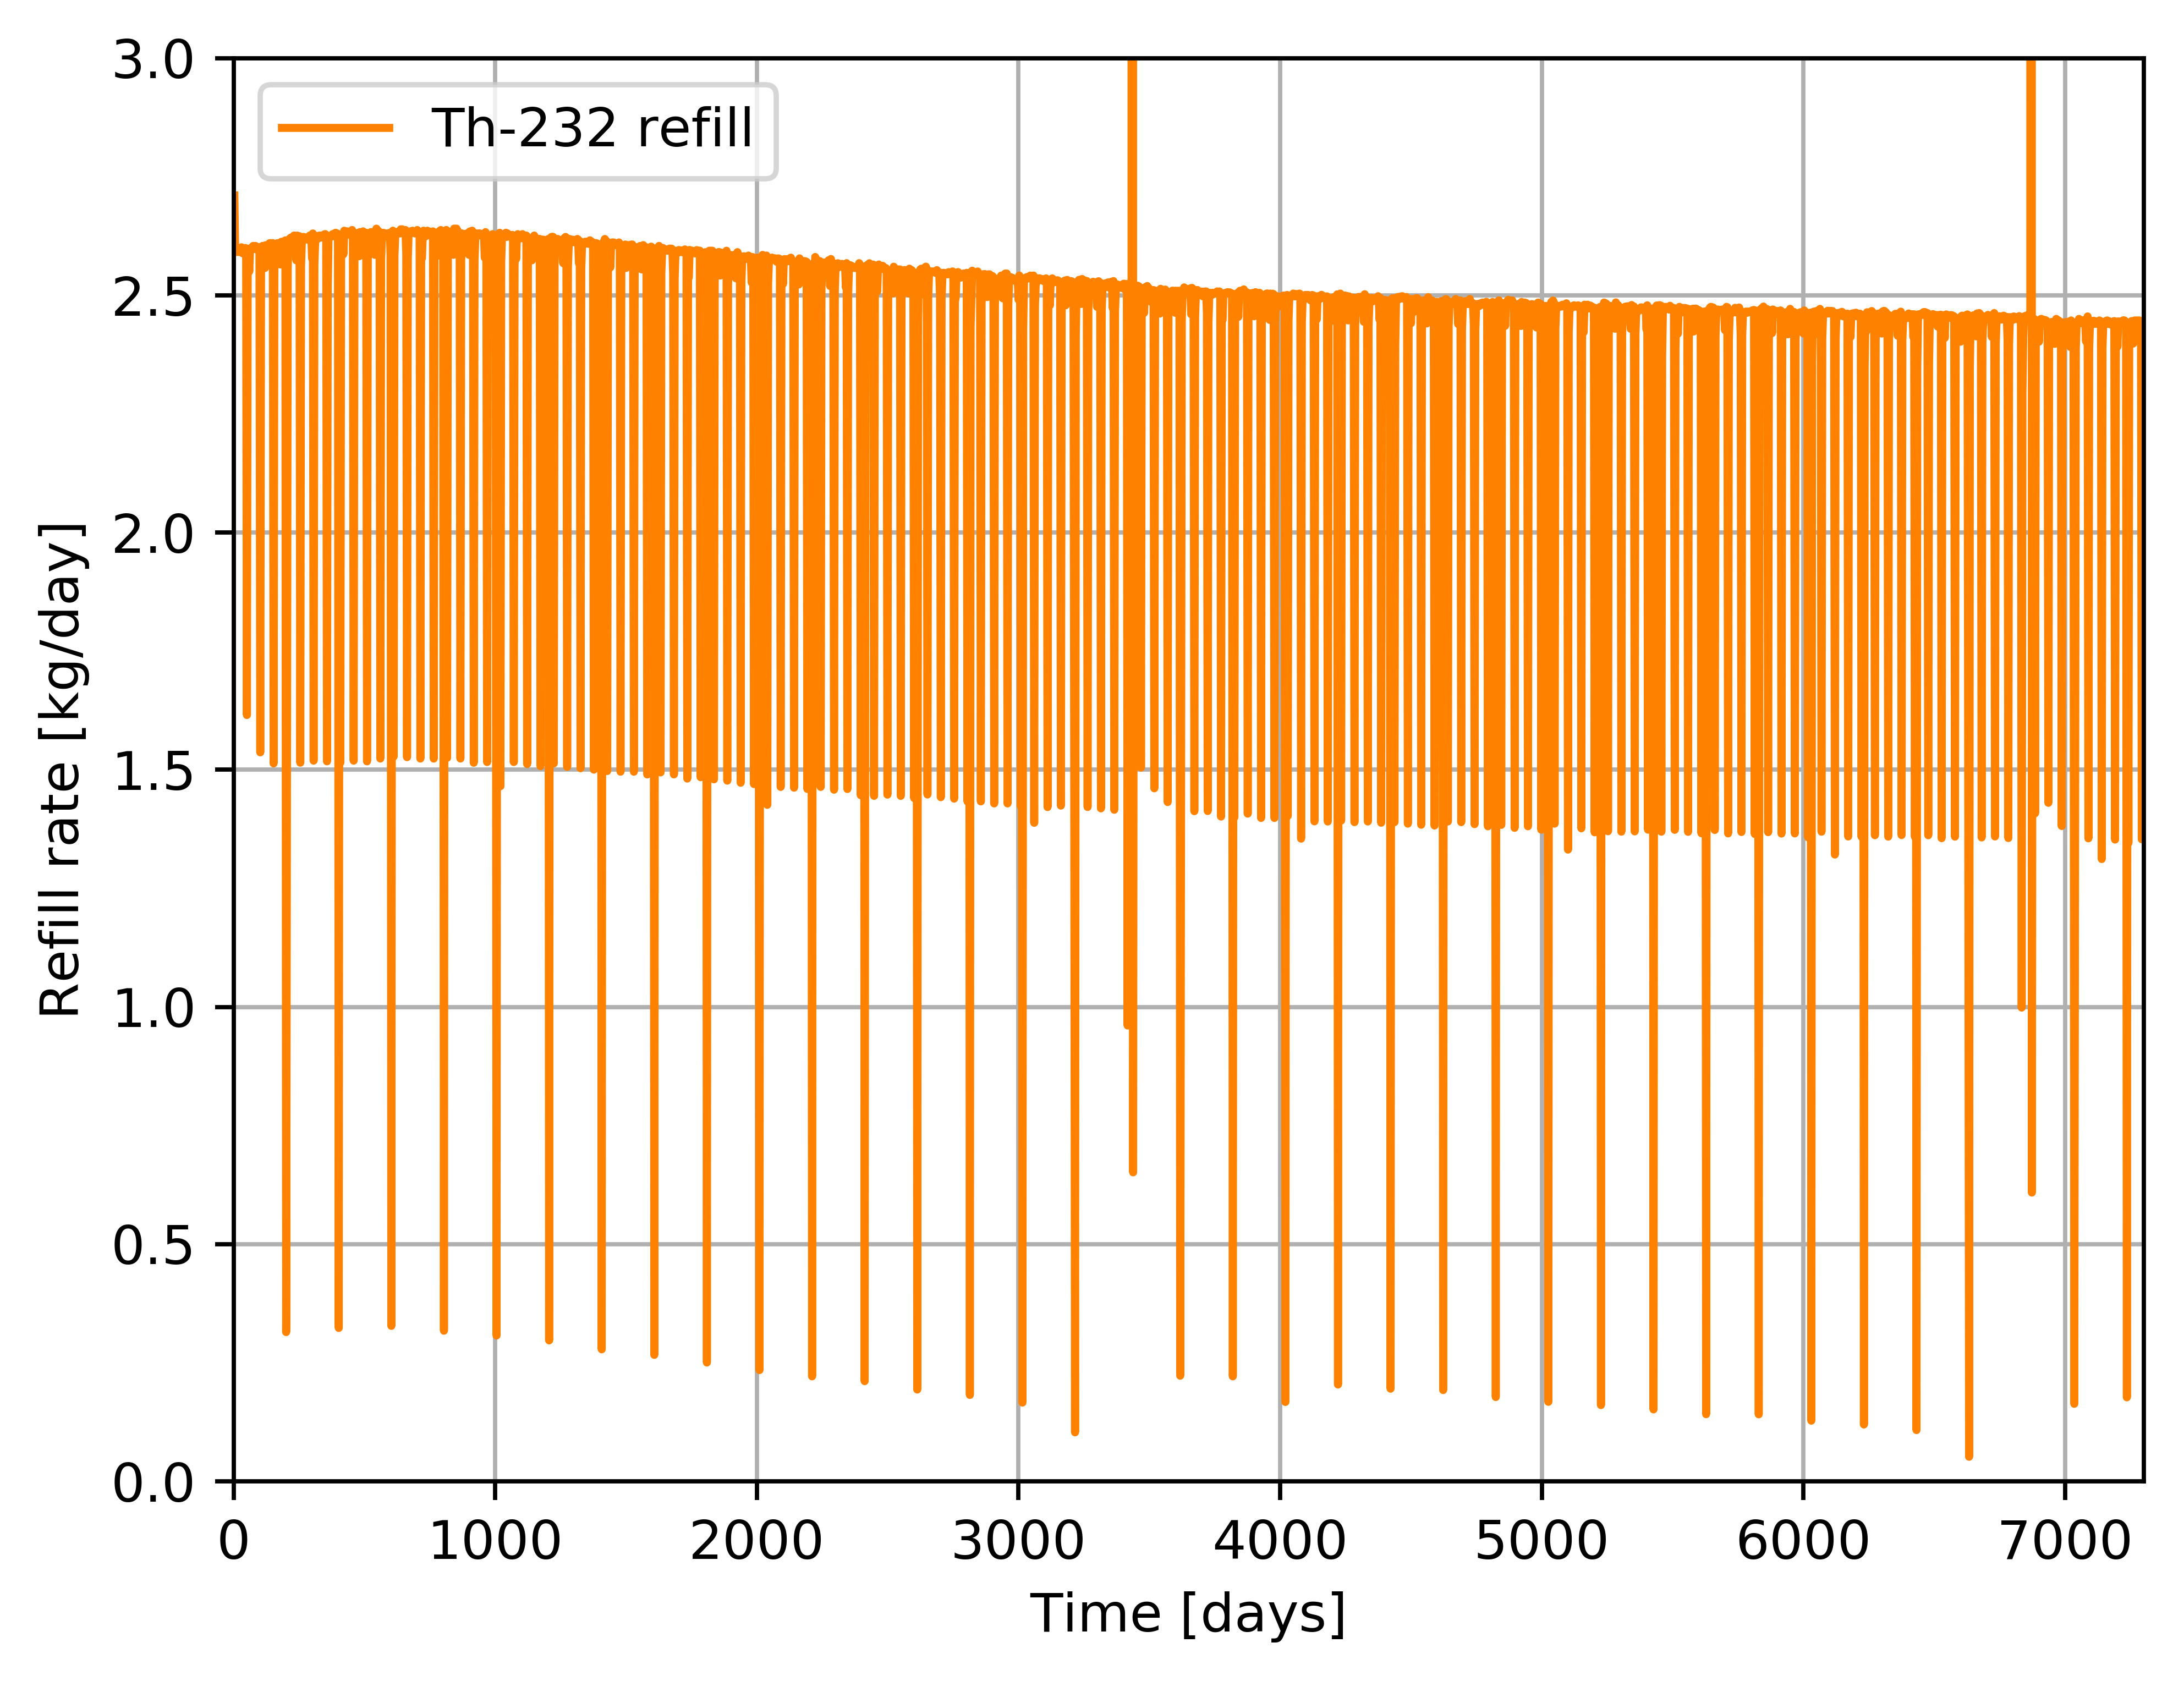
\includegraphics[width=\textwidth]{Th_refill_rate.png} 
      \vspace{-1.5em}
  \caption{$^{232}$Th feed rate over 20 years of \gls{MSBR} operation.}
    \vspace{-0.6em}
  \label{fig:th_refill}
\end{figure}
\begin{figure}[htp!] % replace 't' with 'b' to force it to 
  \centering
    \vspace{-0.3em}
  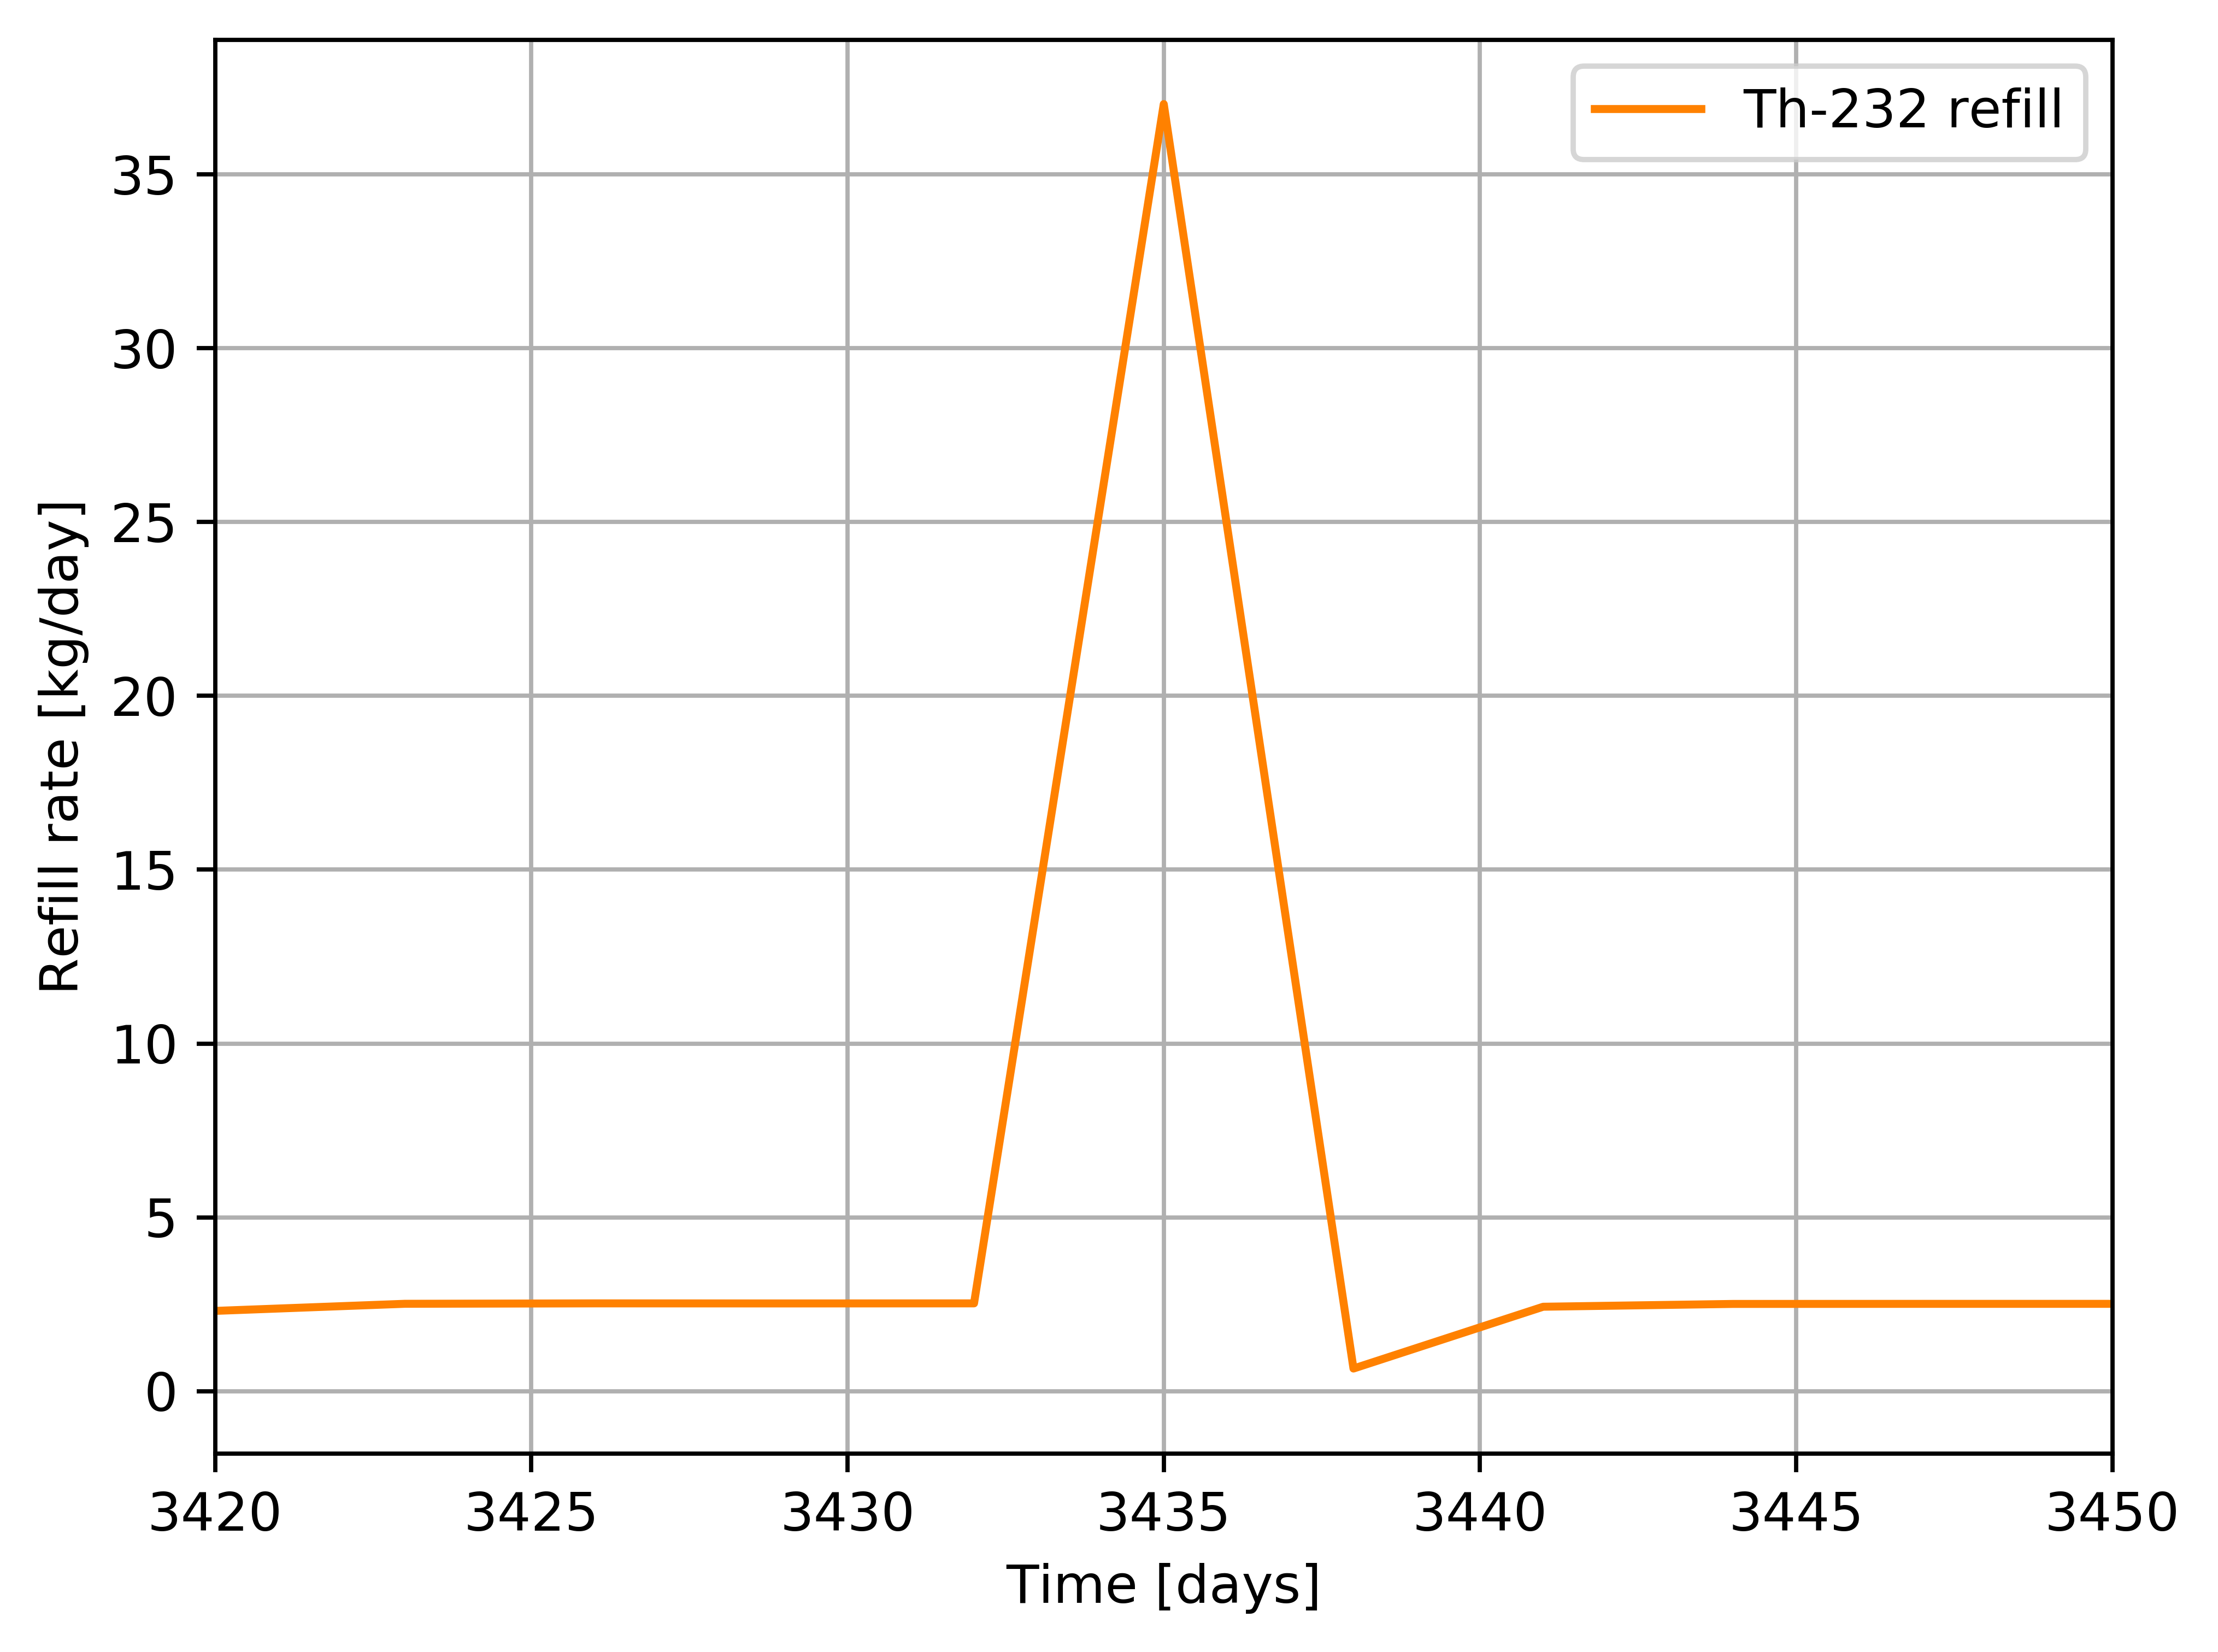
\includegraphics[width=\textwidth]{Th_refill_rate_spike.png} 
      \vspace{-1.5em}
  \caption{$^{232}$Th feed rate spike caused by strong absorbers (Rb, Sr, Cs, Ba) removal.}
    \vspace{-0.6em}
  \label{fig:th_refill_spike}
\end{figure}
\FloatBarrier
